%\documentclass[twoside,openright,a4paper,11pt]{book}
%
%
\usepackage[utf8]{inputenc}
\usepackage[francais]{babel}
\usepackage[T1]{fontenc}

\addto\captionsfrench{\def\tablename{\textsc{Tableau}}}% pour avoir TABLEAU et pas TABLE dans les légendes des tableaux

%%%%%%% MISE EN PAGES %%%%%%
\usepackage{geometry}
\geometry{outer=2cm,inner=3cm,top=3cm}

\setcounter{tocdepth}{3}     % Dans la table des matieres
\setcounter{secnumdepth}{3}  % Avec un numero.
\usepackage{setspace}

\usepackage{fancyhdr}	% marge en haut et en bas
\pagestyle{fancy}

\fancyhead{}	% vide l'entête
\fancyfoot{} % vide le pied~de~page

\fancyhead[RO]{\leftmark}
\fancyhead[LE]{\rightmark}
\fancyfoot[C]{\thepage}	% numéro de page en bas au centre

\renewcommand{\headrulewidth}{0.4pt} % épaisseur du trait en haut
\renewcommand{\footrulewidth}{0.4pt} % épaisseur du trait en bas

\fancypagestyle{mypagestyle}{%
    \fancyhead{}	
    \fancyfoot{} 
    \fancyfoot[C]{\thepage}
    \renewcommand{\headrulewidth}{0.4pt} 
	\renewcommand{\footrulewidth}{0.4pt} 
}

\fancypagestyle{couvertureAbstract}{%
    \fancyhead{}	
    \fancyfoot{} 
    \fancyfoot[C]{}
	\renewcommand{\headrulewidth}{0pt} 
	\renewcommand{\footrulewidth}{0pt} 
}
%
\usepackage{layout}
\usepackage{tocbibind} % include tableofcontent in itself

%%%%%% PAGE DE GARDE %%%%%%

\geometry{outer=2cm,inner=3cm,top=3cm}
\usepackage[scaled]{helvet} % font used on cover (Helvetica)
\usepackage{eso-pic} % to set background picture
\usepackage{multicol} % for back cover (abstracts)
\usepackage{graphicx} % to include logos
\usepackage{tikz} % to compose background picture

% Colors (extracted from SPI's template)
\definecolor{boxcolor1}{rgb}{0.91373,0.92941,0.87451}
\definecolor{boxcolor2}{rgb}{0.94902,0.93333,0.91373}
\definecolor{boxcolor3}{rgb}{0.76078,0.87843,0.17647}
\definecolor{headercolor}{rgb}{0.94118,0.30980,0.17255}
\definecolor{namecolor}{rgb}{1.0,0.4,0.0}
\definecolor{titlecolor}{rgb}{0.19216,0.51765,0.60784}
% Also used: gray, teal (predefined by xcolor package, usually loaded by document class)

% Cover environment, to keep changes local
\newenvironment{cover}{%
  \fontfamily{phv}\selectfont % Select Helvetica font
  \pagestyle{empty} % No page number
}{
  \addtocounter{page}{-1}
  \cleardoublepage
}

% Macro for background common to front and back
\newcommand{\tikzBG}{%
  \path (0,0) rectangle (1,1);
  %TODO: You should adjust the bottom height of the following rectangle to fit your abstract's length
  \path [fill=boxcolor1] (.0571,.11) rectangle (.481,.963); 
  \path [fill=boxcolor2] (.4333,.697) rectangle (.9048,.7475);
  \path [fill=boxcolor2] (.4333,.7811) rectangle (.9048,.8316);
  \path [fill=boxcolor2] (.4333,.8687) rectangle (.9048,.9192);
  \path [fill=boxcolor3] (.0571,.7879) rectangle (.5762,.8316);
  \node[inner sep=0pt] at (0.2285,0.8788) [above left] {%
    
\includegraphics[height=.0707\paperheight,keepaspectratio]{./figures/logo/logo_unb.png}};
  \node[inner sep=0pt] at (0.6667,0.8788) [above right] {%
    
\includegraphics[height=.0808\paperheight,keepaspectratio]{./figures/logo/logo_ecn_color.png}};
  \node at (.0571,.8316) [above right,color=headercolor] {%
    \fontsize{29}{35}\selectfont\bfseries Th\`ese de Doctorat};
}

% Macro for repeated information (to avoid insconsistency)
%TODO: fill in with no formatting but desired case
\newcommand{\firstName}{Jean-Rémy}
\newcommand{\surname}{Gloaguen}
\newcommand{\thesisTitle}{Estimation du niveau sonore de sources d'intérêts au sein de mixtures sonores urbaines : application au trafic routier}

%%%%%%% SYMBOLES %%%%%
\usepackage{tipa}	% pour avoir l'accent concave
\usepackage{lmodern}	% pour les guillemets
\usepackage{gensymb}	% pour les degrés
\usepackage{enumitem}	% pour changer le symbole de l'item (\begin{itemize}[label=$\bullet$])

%%%%%%% EQUATION %%%%%%
\usepackage{amssymb}
\usepackage{amsmath}
\usepackage{fancybox}
\usepackage{xfrac}	% fraction de type "1/4"
\usepackage{cases}	% système équation
\usepackage[overload]{empheq}
\usepackage{bm}		% pour mettre en gras .
\usepackage{units} 	% x/y barre latérale pour les fractions
%
%%%%%%% FIGURE %%%%%%
\usepackage{subfigure}	% utiliser subfigure
\usepackage{float}	% utiliser H dans les figures
%
%%%%%% TABLEAUX %%%%%%
\usepackage{array,multirow,makecell}
%\addto\captionsfrench{\def\tablename{\textsc{Tableau}}}% pour avoir TABLEAU et pas TABLE dans les légendes des tableaux
\usepackage{colortbl} % pour avoir des lignes colorées dans les tableau
%\usepackage{slashbox} % pour les \backslashbox
%\usepackage{subcaption}
\usepackage{hhline}	% pour les lignes horizontales 
\usepackage{tabularx} % permet itemize dans les cellules
\usepackage{booktabs}
\usepackage{longtable}	% pour les tableaux longs

\newcolumntype{L}[1]{>{\raggedright\let\newline\\\arraybackslash\hspace{0pt}}m{#1}}
\newcolumntype{C}[1]{>{\centering\let\newline\\\arraybackslash\hspace{0pt}}m{#1}}
\newcolumntype{R}[1]{>{\raggedleft\let\newline\\\arraybackslash\hspace{0pt}}m{#1}}

%%%%% ALGORITHME %%%%%
\usepackage{algorithm}
\usepackage{algorithmic}

%%%%% BIBLIO %%%%%
\usepackage[fixlanguage]{babelbib}
\selectbiblanguage{french}
\usepackage{breakcites}	% pour couper les références en bout de ligne

%%%%% APPENDICES %%%%%%%
\usepackage[toc,page]{appendix}

%%%%%%%%%%%%%%%%%%%%%
\usepackage{url}	% gérer les adresses www.
\linespread{1.2}	% interligne

\cleardoublepage
%
%\begin{document}
%%%%%%%%%%%%%%%%%%%%%%%%%%%%%%%%%%%%%%%%%%%%%%%%%%%%
\chapter{La factorisation en matrices non-négatives}
Ce chapitre propose de détailler le fonctionnement de la factorisation en matrices non-négatives. Les principes généraux sont dans un premier temps détaillés, puis les différentes approches de cette méthode sont explicités.

\section{Principe de la NMF}
La factorisation en matrice non-négative (abrégé NMF pour \textit{Non-negative Matrix Factorization} en anglais) est une technique d'approximation linéaire visant à décomposer une matrice $\textbf{V}$ non-négative de dimensions $F \times N$ en un produit de deux matrices tel que

\begin{equation}
\textbf{V} \approx \textbf{WH}
\end{equation}

où $\textbf{W}$ et $\textbf{H}$ sont deux matrices, également non-négatives, de dimensions respectives $F \times K$ et $K \times N$, appelées \textit{dictionnaire} et matrice d'\textit{activation}. Le choix du rang de factorisation $K$ est le plus souvent déterminé afin que la relation $F \times K + K \times N << F \times N$ soit respectée. Dans ce cas, la NMF est une méthode d'approximation dite de faible rang car elle permet alors la réduction de la dimensionalité des données. Par sa contrainte de non-négativité, la NMF permet d'assurer que les éléments du dictionnaires appartiennent bien tous au même domaine non-négatif que les données d'observation $\mathbf{V}$, et donc de son interprétabilité. Seules des combinaisons additives ne sont possibles dans le produit $\mathbf{WH}$. Il n'est alors pas possible de soustraire d'informations. En cela, la NMF réalise alors une représentation dite \og par partie \fg{}. Ainsi, chaque colonne $n$ de la matrice $\mathbf{V}$ peut donc être approximée par la somme des éléments de $\mathbf{W}$ pondérés par la colonne $n$ de la matrice $\mathbf{H}$ : 

\begin{equation}
\mathbf{v_n} = \mathbf{Wh_n}
\end{equation}

où les caractères minuscules représentent des vecteurs colonne et $n$ est une trame temporelle. Les majuscules résument des matrices. $\mathbf{W}$ est alors composé d'un ensemble de parties élémentaires (exemple en figure~\ref{fig:ex_NMF}). 

\begin{figure}[t]
\centering
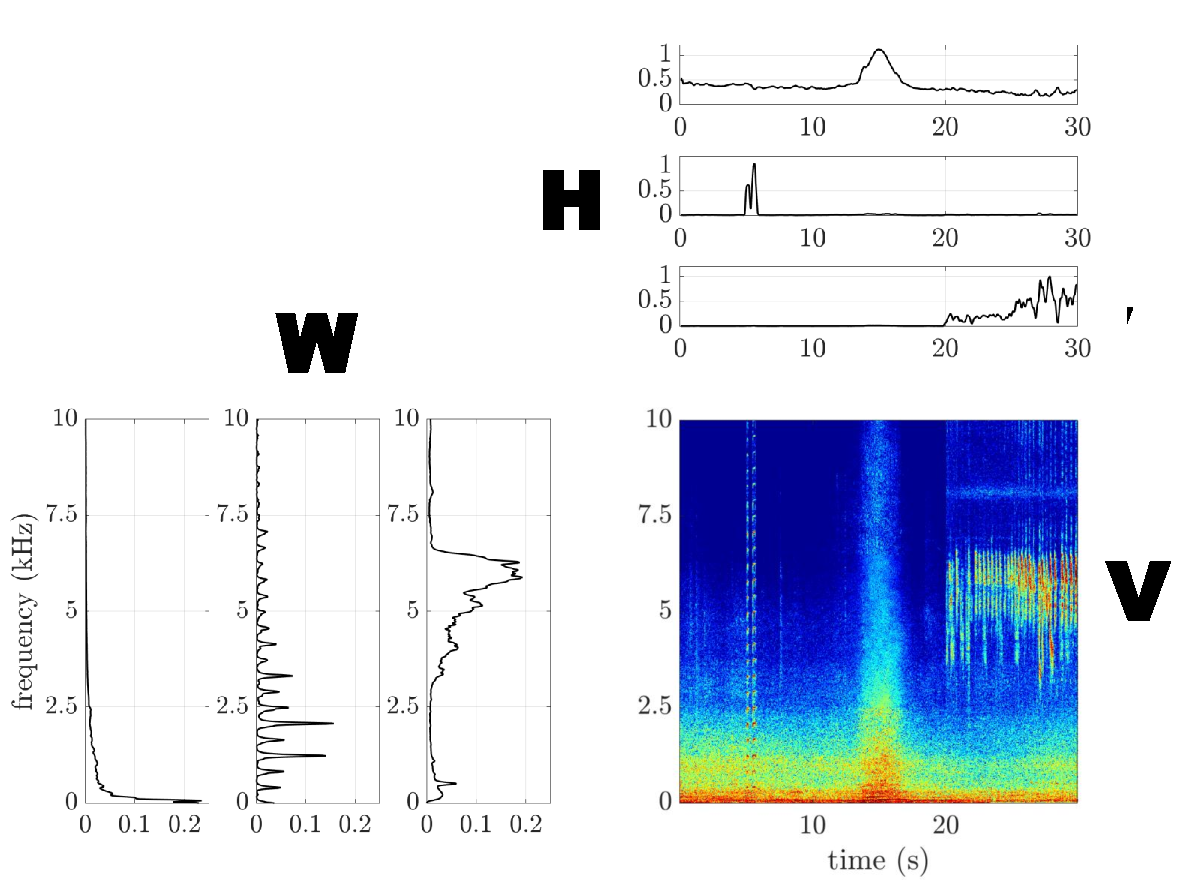
\includegraphics[width=.5\textwidth]{./figures/NMF/schema_introduction_nmf.pdf}
\caption{Exemple d'une NMF pour un signal audio de mixture urbaine composé de 3 sources sonores (dans l'ordre d'apparition klaxon, passage de voiture et oiseaux). $\mathbf{W}$ et $\mathbf{H}$ sont constitués de 3 bases (K = 3).}
\label{fig:ex_NMF}
\end{figure}


Cette méthode est assimilable aux méthodes de factorisation comme l'Analyse en Composantes Principales, où la contrainte de non-négativité est remplacée par une contrainte d'orthogonalité entre les matrice $\mathbf{W}$ et $\mathbf{H}$, ou l'Analyse en Composantes Indépendantes où l'indépendance entre chaque composante est supposée mais où la négativité des données est toutefois possible. \\


Si la NMF fut introduite pour la première fois par Paatero et Tapper \cite{paatero_positive_1994} en 1994 (mais sous le nom de \textit{Positive Matrix Factorization}), elle doit sa popularité aux travaux de Lee et Seung \cite{lee_learning_1999} dont les résultats furent publiés dans la revue \textit{Nature} en 1999. La NMF a ensuite trouvé de nombreuses applications dans des domaines variés 
(imagerie \cite{guillamet_introducing_2003} \cite{monga_robust_2007}, traitement de texte \cite{xu_document_2003} \cite{berry_email_2005}, biologie \cite{gao_improving_2005} \cite{chen_constrained_nodate}, gastronomie \cite{hawkins_clustering_2006} ou bien encore pour la recommandation de contenus audio-visuelle \cite{luo2014efficient}). Dans le domaine de l'audio, c'est Smaragdis et Brown \cite{smaragdis_non-negative_2003} qui furent les premiers à l'utiliser dans le cas de la transcription d'un morceau de musique polyphonique. Le dictionnaire $\mathbf{W}$ est alors constitué d'un ensemble de spectres résumant les notes présentes dans le morceau de musique et les activateurs $\mathbf{H}$ résument l'évolution temporelle de chacun des spectres. De manière plus générale, pour un signal audio quelconque, la NMF consiste à approximer son spectrogramme de puissance, obtenu, par exemple, par une Transformée de Fourier à Court Terme, à l'aide du dictionnaire $\textbf{W}$ constitué d'un ensemble de spectres provenant des différentes sources sonores présentes dont leur amplitude est pondérée temporellement par les activateurs $\textbf{H}$. 

De nombreuses applications de la NMF furent trouvées pour des signaux musicaux et contenant de paroles pour les tâches de la détection et la reconnaissance de source, de la classification de signaux audio, de débruitage et de séparation de sources sonores. Des exemples plus récents ont utilisé la NMF pour des signaux environnementaux, c'est-à-dire les signaux qui ne sont ni musicaux ni de parole. 
 CITATION avec un peu plus de détaille sur le fonctionnement

\section{Fonction coût et familles de divergences}

Le problème à résoudre lors d'une NMF revient à celui d'un problème de minimisation : il faut trouver la combinaison optimale de $\mathbf{WH}$ qui sera la plus proche de $\mathbf{V}$. Cela se traduit mathématiquement par la relation
 
\begin{equation}\label{eq:D(V-WH)}
\text{min}~D\left(\textbf{V} \vert\vert \textbf{WH}\right) \quad \text{avec} \quad \mathbf{W} \geq 0, \mathbf{H} \geq 0 
\end{equation}

$D\left(\textbf{V} \vert\vert \textbf{WH}\right)$ est alors une mesure de similarité appelée \textit{fonction coût} qui peut appartenir à différentes familles de divergences. Les plus usuelles sont les divergences de Csiszar \cite{cichocki2006csiszar} et de Bregman \cite{bregman_relaxation_1967} \cite{dhillon_generalized_2005}. Cette dernière famille de divergences est la plus couramment utilisée dans le cadre de la NMF. Elle se définit, dans un sous-ensemble convexe $S$ d'un espace de Hilbert, comme : 

\begin{equation}\label{eq:Bregdiv}
D_{\Phi}(\textbf{x}\vert\vert \textbf{y}) = 
\mathbf{\Phi}(\mathbf{x}) - \mathbf{\Phi}(\mathbf{y}) - 
\langle\mathbf{x}-\mathbf{y},\nabla\mathbf{\Phi}(\mathbf{y})\rangle
\end{equation}

où  $\mathbf{x} = (x_1, x_2, \dots x_N)$ et $\mathbf{y} = (y_1, y_2, \dots y_N)$ sont deux distributions, $\mathbf{\Phi}$ est une fonction continue dérivable et strictement convexe définit en $\mathbb{R}^+$, $\nabla\mathbf{\Phi}(\mathbf{y})$ est le gradient de $\mathbf{\Phi}$ en $\mathbf{y}$ et $\langle .,.\rangle$ est le produit scalaire hermitien. L'équation~(\ref{eq:Bregdiv}) peut être décomposable élément par élément : 

\begin{equation}
D_{\Phi}(\mathbf{x}\vert\vert \mathbf{y}) = \sum_{n=1}^N d_{\Phi}(x_n\vert y_n)
\end{equation}

avec $d_{\Phi}(x_n\vert y_n)$, la mesure de similarité entre deux scalaires et $\mathbf{\Phi(x)} = \sum_{n=1}^N \phi(x_n)$. L'équation \ref{eq:Bregdiv} se résume alors à une somme des divergences entre les composantes des distributions $\mathbf{x}$ et $\mathbf{y}$ :

\begin{equation}\label{eq:divBregWise}
D_{\Phi}(\textbf{x}\vert\vert \textbf{y}) = \sum_{n=1}^N \phi(x_n)-\phi(y_n)-\phi'(y_n)(x_n-y_n).
\end{equation}

La divergence de Bregman peut ainsi se décomposer pour chaque composante de $\mathbf{V}$ et $\mathbf{WH}$, 

\begin{equation}\label{eq:similarite2}
D\left(\textbf{V} \vert\vert \textbf{WH} \right) = \sum_{f = 1}^{F} \sum_{n = 1}^{N} d_{\phi}
\left(\textbf{V}_{fn} \vert \left[ \textbf{WH} \right]_{fn} \right).
\end{equation}


Cette divergence possède plusieurs propriétés : 

\begin{enumerate}
\item \textbf{Non-négativité} : $d_{\phi}(x\vert y) \geq 0$.

\item \textbf{Séparabilité} : si $d_{\phi}(x\vert y) = 0$ alors $x = y$

\item \textbf{Convexité} : $D_{Br}(\textbf{x}\vert\vert \textbf{y})$ est une fonction réelle strictement convexe pour le 1\ier{} argument mais pas nécessairement pour le second.

\item \textbf{Linéarité} : pour deux fonctions convexes, réelles $\phi_1$ et $\phi_2$,  $d_{\alpha \phi_1 + \beta \phi_2}(x\vert y) = \alpha d_{\phi_1}(x\vert y)+\beta d_{\phi_2}(x\vert y)$ où $\alpha$ et $\beta \in \mathbb{R}^+$.

\item \textbf{Dualité} : pour la fonction convexe conjuguée $\phi^{\ast}$, $d_{\phi^{\ast}}(y^{\ast}\vert x^{\ast}) = d_{\phi}(y \vert x)$
\end{enumerate}

Si la propriété de non-négativité en fait une famille adaptée pour la NMF, celle de convexité implique qu'il n'est possible que de déterminer un minimum local et donc pas nécessairement la solution exacte au problème énoncé.


\section{Une sous-classe des divergences de Bregman : la $\beta$-divergence}

Dans \cite{banerjee2005clustering}, les auteurs démontrent qu'à chaque divergence de Bregman est associée une famille exponentielle unique: 

\begin{equation} \label{eq:modele_disp_exp}
p\left(x\vert \theta,\lambda\right) = h(x,\lambda) \exp\left[\lambda^{-1}\left(\theta x-\psi(\theta) \right)\right], 
\end{equation}

avec $h(x,\theta) $, la fonction de base, $\theta$, le paramètre normal (ou canonique), $\lambda$, celui de la dispersion et $\psi$ celui de la normalisation. Les fonctions $\lambda(\theta)$ et $\phi(\mu)$ sont alors considérés comme des fronction conjuguées dual tout comme le paramètre $\theta$ est la conjugué de $\mu$. On a alors comme relations

\begin{equation}\label{eq:mu1}
\mu(\theta) = \frac{d\lambda(\theta)}{d\theta}
\end{equation}
\begin{equation}\label{eq:mu2}
\theta(\mu) = \frac{d\phi(\mu)}{d\mu}
\end{equation}

Il est alors possible de relier les paramètre $\theta$ et $\mu$, à travers la fonction de variance $v(\mu)$, 

\begin{equation}
\frac{d\theta}{d\mu} = v(\mu)^{-1}
\end{equation}

qui est, elle-même, relié à la variance de la distribution de $x$ par le paramètre de dispersion $\lambda$, 

\begin{equation}
Var(x) = \lambda v(\mu)
\end{equation}

Il est alors possible d'exprimer chaque divergence de Bregman sous la forme 

\begin{equation} \label{eq:g_exp}
p\left(x\vert \theta,\lambda\right) = g(x,\varphi) \exp\left(-\lambda^{-1} d_{\theta}(x,\mu) \right), 
\end{equation}

où $d_{\theta}(x,\mu)$ est la divergence de Bregman définit par l'équation \ref{eq:Bregdiv}. Un cas remarque de distribution est la distribution de Tweedie \cite{jorgensen_exponential_1987} qui relie la variance à la moyenne (ou espérance) de la distribtion $x$ par une relation polynomiale \cite{yilmaz_alpha/beta_2012}, 

\begin{equation}
v(\mu) = \mu^{p}.
\end{equation}

Des relations \ref{eq:mu1} et \ref{eq:mu2}, avec un changement de variable $p = 2-\beta$, la fonction $\phi_{\beta}(\mu)$ est déterminée : 

\begin{subequations}\label{eq:gamma_beta}
\begin{numcases}{\phi_{\beta}(\mu)=}
    \frac{\mu^{\beta}}{\beta(\beta-1)}-\frac{\mu}{\beta-1}+\frac{1}{\beta}, & $\beta \in \mathbb{R} \backslash \lbrace 0,1\rbrace$,\label{eq:phi}\\
    -\log \mu + \mu - 1, & $\beta = 0$,\label{eq:phiIs}\\
    \mu\log \mu - \mu + 1, & $\beta = 1$.\label{eq:phiKL}
\end{numcases}
\end{subequations}

Une distribution gaussienne de moyenne $\mu$ et de variance $\sigma^2$, 

\begin{equation}
p(x \vert \theta, \lambda) = \frac{1}{\sqrt{2 \pi \sigma^2}}\exp\left(-\frac{1}{2} \left(\frac{x-\mu}{\sigma} \right)^2 \right)
\end{equation}

peut alors s'exprimer sous la forme d'une distribution de Tweedie, avec $\beta$ = 2, $g(x, \lambda) = \frac{1}{\sqrt{2 \pi \sigma^2}}$ et $\lambda = \sigma^2$. $d_{2}(\mu)$ correspond alors à la distance euclidienne. Le cas $\beta = 1$ fait apparaitre la divergence de Kullback-Liebler et correspond alors à une distribution de Poisson et $\beta = 0$ exprime la divergence d'Itakura-Saïto  dans une distribution Gamma. Ces distances et divergences, déduites de la distribution de Tweedie, sont alors regroupés dans une sous classe des divergences de Bregman, appelée $\beta$-divergences \cite{hennequin_beta-divergence_2011}. C'est cette famille de divergences qui est le plus couramment utilisé dans le cadre de la NMF.\\

Les détails des calculs se trouvent en annexe \ref{annexe:tweedie}.

\subsection{Définition des $\beta$-divergences}

L'application du système \ref{eq:gamma_beta} à l'équation \ref{eq:divBregWise} pour deux valeurs scalaires $x$ et $y$ donne alors 

\begin{subequations}\label{eq:divBetaGenerale}
\begin{numcases}{d_{\phi_{\beta}}(x\vert y) =}
    \frac{1}{\beta(\beta-1)}(x^{\beta}+(\beta-1)y^{\beta}-\beta xy^{\beta-1}), & $\beta \in \mathbb{R} \backslash \lbrace 0,1\rbrace$\\
    \dfrac{x}{y}-\log \dfrac{x}{y}-1, & $\beta = 0$,\label{eq:def_divIS}\\
    x\log \dfrac{x}{y} - x + y, & $\beta = 1$.\label{eq:def_divKL}
\end{numcases}
\end{subequations}

La figure~\ref{fig:allure-divergence} permet d'illustrer le comportement strictement convexe des divergences pour $\beta \in \left[1,2\right]$. En dehors de cet intervalle, les divergences présentent une partie concave. Dans le reste du document, par soucis de clarté, $d_{\phi_{\beta}}$ est dénommé $d_{\beta}$. \\

\begin{figure}[h]
\centering
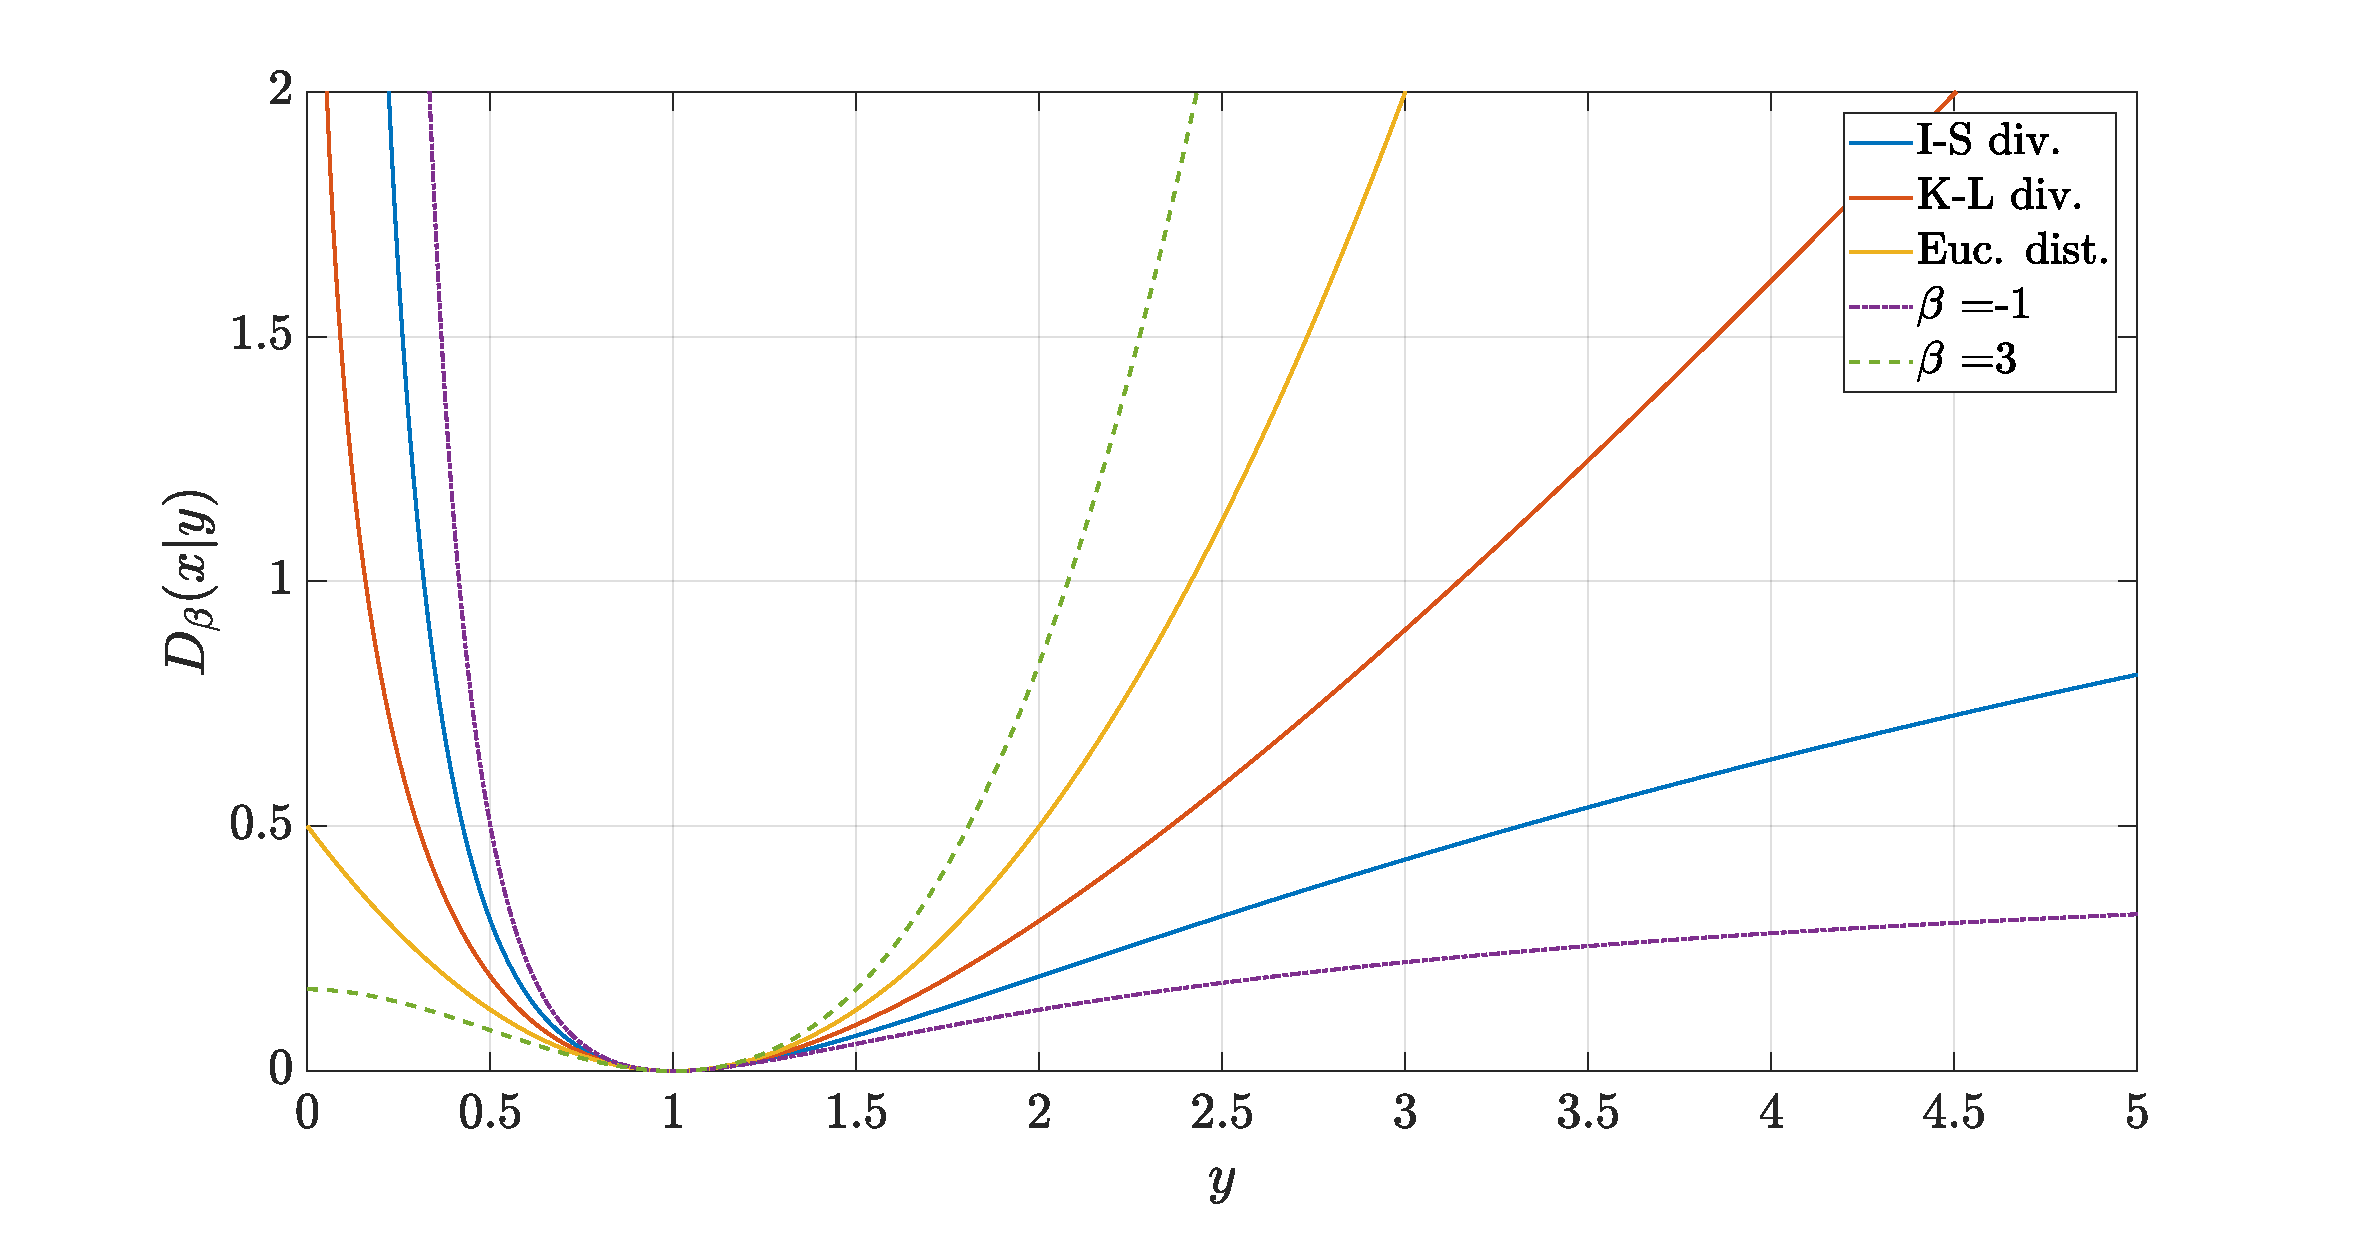
\includegraphics[width=.7\textwidth]{./figures/NMF/betaDiv_exemple01.pdf}
\caption{Évolution des $\beta$-divergences pour un cas simple ($x$ = 1)}
\label{fig:allure-divergence}
\end{figure}

L'équation~\ref{eq:divBetaGenerale} possède trois cas particuliers qu'il est nécessaire de démarquer. 

\subsubsection{Distance euclidienne}
La première divergence remarquable se trouve lorsque $\beta = 2$ en devenant \textbf{la distance euclidienne} (abrégé EUC) : 

\begin{equation}
d_{{2}}(x\vert y) = \dfrac{1}{2}(x-y)^2.
\end{equation}

Cette métrique équivaut à une mesure de similarité entre les points $x$ et $y$ et se révèle très sensible aux grandes variations entre eux en raison de la préscence de la puissance carré. En plus des propriétés des divergences de Bregman, la distance euclidienne en possède 2 autres : 
\begin{enumerate}

\item \textbf{Symétrie} : $d_{\beta}(x \vert y ) = d_{\beta}(y \vert x)$.

\item \textbf{Inégalité triangulaire} : $d_{\beta}(x \vert y ) \leq d_{\beta}(x \vert z ) + d_{\beta}(x \vert z )$.\\
\end{enumerate}

Ajoutons, comme chaque mesure de distance au point $xy$ possède le même poids que les autres points, qu'il est possible, pour la distance euclidienne, de pondérer les distances selon un critère psycho-acoustique, 

\begin{equation}
d'_2(v_{fn} \vert w_{fk} h_{kn}) = g_{v_{fn}} d_2 (v_{fn} \vert w_{fk} h_{kn})
\end{equation}

où $g_{v_{fn}}$ est une pondération liée à l'énergie de $v_{fn}$. Cette pondération permet de prendre en compte dans l'erreur de reconstruction, les points temps-fréquences de faibles énergies \cite{virtanen2004separation}. 

\subsubsection{Divergence de Kullback-Leibler}
L'expression \ref{eq:def_divKL} correspond à \textbf{la divergence de Kullback-Leibler} (ou entropie relative), abrégé K-L, \cite{kompass_generalized_2007}, \cite{cichocki_new_2006} . Elle traduit comment une densité de probabilité, $x$, diverge d'une seconde distribution $y$. En d'autre terme, c'est une mesure de l'information perdu lorsque $y$ est utilisé pour approximer $x$. Ne respectant pas les propriétés de symétrie et d'inégalité triangulaire, elle ne peut pas être considéré comme une distance mais plus plus comme un calcul de similarité. La divergence K-L est un cas remarquable puisqu'elle appartient à la foi aux divergences de Bregman et à une autre famille de divergences: les divergences de Csiszar \cite{cichocki_csiszars_2006}. 

\subsubsection{Divergence d'Itakura-Saïto}
Enfin, l'expression \ref{eq:def_divIS} est celle de \textbf{la divergence d'Itakura-Saïto} \cite{itakura1968analysis} \cite{bertin_les_2009}. Cette divergence possède une propriété unique d'\textit{invariance d'échelle} qui se traduit par 

\begin{equation}\label{eq:scale_IS}
d_{0}(\lambda x \vert \lambda y) = d_{0}(x \vert y).
\end{equation}

Ce rapport signifie que le même poids est attribué entre les fortes et les faibles valeurs de $x$. Ainsi, la divergence aux faibles puissances entre $\textbf{V}$ et $\textbf{WH}$ aura la même importance que dans les fortes puissances. La relation \ref{eq:scale_IS} peut être étendu à l'ensemble de $\beta$,  

\begin{equation}
d_{\beta}(\lambda x \vert \lambda y) = \lambda^{\beta}d_{\beta}(x \vert y)
\end{equation}


Pour les cas où $\beta > 0$, la divergence est plus influencé par les composantes de fortes amplitudes et moins par les composantes de faibles puissances. À l'inverse, dans les cas où $\beta < 0$, les composantes ayant une faible amplitude ont plus une grande prépondérance. Cette particularité, d'après \cite{fevotte_nonnegative_2009}, est intéressante dans le cadre de signaux audio, et dans leur étude les signaux audio musicaux qui possède une forte dynamique et dont la puissance décroit exponentiellement. Une faible $\beta$ permet alors de mieux prendre en compte les composantes d'amplitudes moindre dans la reconstruction du signal. Enfin, il n'est pas nécessaire de se restreindre aux divergences bien connues:  \cite{vincent2010adaptive} a utilisé la NMF dans le cadre de la transcription de signaux musicaux et a déterminé un résultat optimal pour $\beta$ = 0,5. \\

\subsection{Autres familles de divergences}
Si on s'est attardé à décrire longuement la $\beta$-divergence, d'autre familles de divergence peuvent être utilisé pour la NMF notamment celle appartenant aux divergences de Csiszar ou appelée $f$-divergence. Cette famille est toutefois moins utilisée que celle de Bregman. Elle se définit comme 

\begin{equation}
D_{\Psi} (\mathbf{x} \Vert\mathbf{y}) = \mathbf{x} \mathbf{\Psi} \left( \frac{\mathbf{x}}{\mathbf{y}}\right)
\end{equation}

Elle intègre la distance de variation totale ($\psi(x) = \frac{1}{2}\vert x-1 \vert $), la divergence $\chi^2$ ($\psi(x) = (x-1)^2$), la distance d'Hellinger ($\psi(x) = (\sqrt{t}-1)^2$), les divergences $\alpha$ d'Amari $\left(\psi(x) = \frac{4}{1-\alpha^2} \left(1-x^{(1+\alpha)/2} \right)\right)$ et la divergence de Kullback-Leibler ($\psi(x) = x\log (x)$). Cette dernière est la seule à appartenir aux divergence de Bregman et de Csiszar et donc à posséder leurs propriétés communes. Elle possède plusieurs propriétés (non-négativité, unicité de la solution, symétrie, convexité, dépendance) qui sont détaillé dans \cite{csiszar2004information}.

Enfin, une proposition de généralisation des familles de divergences peut être trouvée dans \cite{cichocki_generalized_2011} où les auteurs généralisent les $\alpha$ et les $\beta$ divergences à travers l'équation  \ref{eq:expression_gen_alpha_beta} 

\begin{equation}\label{eq:expression_gen_alpha_beta}
D_{a, b}(x \vert y) = \frac{1}{a b}\left(x^{a}y^{\beta}- \frac{a}{a+b}x^{a + b}-\frac{b}{a+b}y^{a+b} \right).
\end{equation}

La valeur des coefficients $a$ et $b$ permet alors de d'obtenir soit des $\beta$-divergences ($a = 1$) ou des $\alpha$-divergence ($a+b = 1$) mais également de nouvelles divergences. L'intérêt d'étendre les familles et les divergences est multiple : elle permet de déterminer de nouveaux algorithmes de mises à jours dont les convergences peuvent être plus rapides et elles permettent d'offrir de nombreuses fonctions coûts permettant ainsi de les adapter au problème initial rencontré. Dans le cadre de ce travail, nous nous restreignons aux $\beta$-divergences. Ce choix est notamment motivé par la popularité de ces divergences et aux nombreuses références dans la littérature qui s'y réfèrent.

\section{Mise à jour des formes de \textbf{W} et de \textbf{H}}

La minimisation de la divergence $D(\mathbf{V} \Vert \mathbf{WH})$ entre $\mathbf{V}$ et $\mathbf{WH}$ revient à un problème d'optimisation la forme des matrices $\mathbf{W}$ et $\mathbf{H}$ évoluent itérativement à l'aide d'algorithmes de mises à jour qui dépendent du choix de $\beta$. 

Sont présentés ici, les algorithmes multiplicatifs des matrices de $\mathbf{W}$ et $\mathbf{H}$ les plus couramment utilisées. Ces algorithmes garantissent que la contrainte de non-négativité soit bien respectée.

\subsection{Algorithme heuristique par descente de gradient}

Dans leur premier article consacré à la NMF, Lee et Seung \cite{lee_learning_1999} propose une première formulation des algorithmes de mises à jours, sans toutefois expliciter leur origine,  pour $\beta  \in \lbrace 1,2 \rbrace$.

\begin{subequations}\label{eq:WHupdateGD}
\begin{align}
\textbf{W}^{(i+1)} &\leftarrow \textbf{W}^{(i)}.\frac{\left[\left(\textbf{W}^{(i)}\mathbf{H} \right)^{(\beta-2)}.\textbf{V} \right]\textbf{H}^T}{\left[\textbf{W}^{(i)}\mathbf{H} \right]^{(\beta-1)}\textbf{H}^T}\\
\textbf{H}^{(i+1)} &\leftarrow \textbf{H}^{(i)}.\frac{\textbf{W}^T \left[\left(\textbf{WH}^{(i)} \right)^{(\beta-2)}.\textbf{V} \right]}{\textbf{W}^T \left[\textbf{WH}^{(i)} \right]^{(\beta-1)}}
\end{align}
\end{subequations}

Les termes $A.B$ et $\dfrac{A}{B}$ sont des produits de Hadamard (respecivement multiplication et division terme à terme). La minimisation de la fonction \ref{eq:D(V-WH)} se fait alors alternativement : pour $\mathbf{W}$ fixé, $\mathbf{H}$ est mis à jour, puis $\mathbf{H}$ est fixé et c'est $\mathbf{W}$ qui est mis à jour.

La démonstration de ces algorithmes se fait à l'aide de la méthode de descente de gradient \cite{lee_algorithms_2000}. Cette méthode consiste à faire \og glisser \fg {} une solution temporaire le long de la pente négative d'une fonction $f(x)$ afin de converger vers la solution \cite{kivinen_exponentiated_1994}.

\begin{equation}\label{eq:gradient_descent}
x^{(i+1)} \leftarrow x^{(i)} - \eta^{(i)} \nabla f(x^{(i)})
\end{equation} 

avec $\eta^{(i)}$ le pas d'apprentissage. Dans le cadre de la NMF, pour la distance EUC, les équations \ref{eq:gradient_descent} deviennent

\begin{subequations}\label{eq:WHgradientDescente}
    \begin{align}
     \mathbf{W}^{(i+1)} & \leftarrow \mathbf{W}^{(i)}+\eta_{\mathbf{W}}\left[ \left(\mathbf{V H^T}\right)^{(i)} - \left(\mathbf{W H H^T}\right)^{(i)} \right ] \\
      \mathbf{H}^{(i+1)} & \leftarrow \mathbf{H}^{(i)}+\eta_{\mathbf{H}}\left[ \left(\mathbf{W^TV}\right)^{(i)}-\left(\mathbf{W^T W H} \right)^{(i)}\right ]      
    \end{align}
\end{subequations}

avec $\eta_{\mathbf{W}} = \frac{\mathbf{W}}{\mathbf{WHH^T}}$ et $\eta_{\mathbf{H}} = \frac{\mathbf{H}}{\mathbf{W^TWH}}$, les pas d'apprentissages respectif choisis judicieusement afin d'obtenir les algorithmes de mises à jours\ref{eq:WHupdateGD}. Cette méthode est également développée pour la divergence de Kullback-Leibler dans le même article mais n'est alors pas étendu à l'ensemble de la famille des $\beta$-divergences. La preuve de la convergence des algorithmes est ensuite démontré à l'aide de l'utilisation d'une fonction auxiliaire, voir partie \ref{part:sub_fonction_aux}.


\subsection{Algorithme heuristique multiplicatif}


Cette approche utilise également un algorithme de descente. Proposé par Févotte et al. dans \cite{fevotte_nonnegative_2009}, le principe consiste à exprimer la dérivée (selon $\mathbf{W}$ ou $\mathbf{H}$) de $D(\mathbf{V} \Vert\mathbf{WH})$,  comme la différence de deux fonctions non-négatives tels que $\nabla_{\mathbf{W}/\mathbf{H}} D = \nabla^+_{\mathbf{W}/\mathbf{H}}D-\nabla^-_{\mathbf{W}/\mathbf{H}}D$. La minimisation de la fonction coût \ref{eq:D(V-WH)} se réalise alors en multipliant le point à l'itération précédente par le rapport de la partie négative et de la partie positive de la dérivée à ce point, 

\begin{subequations}
    \begin{align}
     \mathbf{W}^{(i+1)} & \leftarrow \mathbf{W}^{(i)}\frac{\nabla_\mathbf{W}^-D(\mathbf{V}\Vert\mathbf{WH})}{\nabla_\mathbf{W}^+D(\mathbf{V}\vert \vert \mathbf{WH})}\\
     \mathbf{H}^{(i+1)} & \leftarrow \mathbf{H}^{(i)}\frac{\nabla_\mathbf{H}^-D(\mathbf{V}\Vert\mathbf{WH})}{\nabla_\mathbf{H}^+D(\mathbf{V}\Vert\mathbf{WH})}    
    \end{align}
\end{subequations}


menant alors aux équations \ref{eq:WHupdateMM}. 

\begin{subequations}\label{eq:WHupdateMM}
\begin{align}
\textbf{W}^{(i+1)} &\leftarrow \textbf{W}^{(i)}.\left(\frac{\left[\left(\textbf{W}^{(i)}\mathbf{H} \right)^{(\beta-2)}.\textbf{V} \right]\textbf{H}^T}{\left[\textbf{W}^{(i)}\mathbf{H} \right]^{(\beta-1)}\textbf{H}^T}\right)^{\gamma(\beta)}\label{eq:WupdateMM}\\
\textbf{H}^{(i+1)} &\leftarrow \textbf{H}^{(i)}.\left(\frac{\textbf{W}^T \left[\left(\textbf{WH}^{(i)} \right)^{(\beta-2)}.\textbf{V} \right]}{\textbf{W}^T \left[\textbf{WH}^{(i)} \right]^{(\beta-1)}}\right)^{\gamma(\beta)}\label{eq:HupdateMM}
\end{align}
\end{subequations}

avec 

\begin{subequations}\label{eq:gammaGenerale}
\begin{numcases}{\gamma(\beta) =}
    \frac{1}{2-\beta}, & $\beta < 1$, \\
    1, & 1 $\leq \beta \leq 2$,\\
    \frac{1}{\beta-1}, & $\beta > 2$.
\end{numcases}
\end{subequations}


Les équations \ref{eq:WHupdateMM} sont valables pour tout $\beta \in \mathbf{R}$. Enfin, on remarque que dans l'intervalle $\left[1,2 \right]$, l'expression des algorithmes  \ref{eq:WHupdateMM} est la même que celles de \ref{eq:WHupdateGD}. Les parties \ref{part:convergenceMM} et \ref{part:sub_fonction_aux} présentes la preuve de la convergence de cette algorithme ainsi que la formation de la fonction auxiliaire. 

\subsection{Convergences des algorithmes}\label{part:convergenceMM}

Dans le cas de l'algorithme obtenue par descente de gradient ou par l'algorithme heuristique, la preuve de la convergence est obtenue par l'utilisation d'une fonction auxiliaire. Comme l'approximation de la NMF est transposable ($\mathbf{V} \approx \mathbf{WH} \Leftrightarrow \mathbf{V}^T \approx \mathbf{H}^T \mathbf{W}^T$). Il est possible de restreindre l'étude au cas de la mise à jour de $\mathbf{H}$ pour $\mathbf{W}$ fixé. Considérons le problème suivant :  

\begin{equation}
\underset{\textbf{H > 0}}{\text{min}}~C(\mathbf{H}) = D(\mathbf{V} \vert\vert \mathbf{WH})
\end{equation}

avec $\mathbf{W}$ fixé. Ce problème peut être décomposé pour chaque trame temporel

\begin{equation}\label{eq:costFunctionMM}
C(\mathbf{h}) = D(\mathbf{v}\vert\vert \mathbf{Wh}).
\end{equation}

On définit alors la fonction auxiliaire $G(\mathbf{h}\vert \mathbf{h})$ de $C(\mathbf{h})$ avec pour conditions : 
\begin{subequations}\label{eqs:conditionAux}
\begin{align}
C(\mathbf{h}^{\left(i\right)}) &= G(\mathbf{h}^{(i)}\vert \mathbf{h}^{(i)}) \quad \forall~\mathbf{h} \in \mathbb{R}^+_K,\\
C(\mathbf{h}^{(i)}) &\leq G(\mathbf{h}^{(i)} \vert \mathbf{h}^{(i+1)}) \quad \forall~\mathbf{h} \in \mathbb{R}^+_K.
\end{align}
\end{subequations}

La détermination d'un $\mathbf{h}$ optimal est alors déterminée itérativement afin que 

\begin{equation}
\textbf{h}^{(i+1)} = \underset{\textbf{h} \geq 0}{\text{arg min}}~ G(\textbf{h}^{(i+1)}\vert \textbf{h}^{(i)})
\end{equation}
\begin{equation}
C(\mathbf{h}^{(i+1)}) \leq G(\textbf{h}^{(i+1)}\vert\mathbf{h}^{(i)}) \leq G(\textbf{h}^{(i)}\vert\mathbf{h}^{(i)}) = C(\mathbf{h}^{(i)})
\end{equation}

\subsection{Autres approches}

D'autres approches ont été proposés comme la méthode des moindres carrées alternées \cite{cichocki_regularized_2007} \cite{berry_algorithms_2007} qui consiste à minimiser successivement la distance EUC entre $\mathbf{V}$ et $\mathbf{WH}$ en fixant chaque variable alternativement, 

\begin{subequations}\label{eq:als}
\begin{align}
\mathbf{W}^{(i+1)} &= \text{arg}~\underset{\mathbf{W} > 0}{\text{min}}~D\left(\mathbf{V} \vert\vert\mathbf{W}^{(i)}\mathbf{H}^{(i)}\right)\\
\mathbf{H}^{(i+1)} &= \text{arg}~\underset{\mathbf{H} > 0}{\text{min}}~D\left(\mathbf{V} \vert\vert\mathbf{W}^{(i+1)}\mathbf{H}^{(i)}\right)
\end{align}
\end{subequations}

Pour résoudre les équations \ref{eq:als}, Zdunek et Cichocki \cite{zdunek2006non} proposent d'utiliser la méthode de Newton. Lin \cite{lin_projected_2007} utilise la méthode par projection de gradient. Si ces méthodes offres des convergences plus rapide que les algorithmes multiplicatifs; elles sont alourdit par la présence de matrice hessienne et ne permettent pas d'intégrer aussi facilement des contraintes sur $\mathbf{W}$ ou $\mathbf{H}$. De plus, ces méthodes de résolutions ne sont adaptées que pour des distances euclidiennes ou de Kullback-Leibler se qui restreint les possibilités d'adapter les fonctions coûts aux problèmes.\\

%%%%%%%%%%%%%%%%%%%%%%%%%%%%%%%%%%%%%%%%%%%%%%%%%%%%%%%%%


%Dans le cas de la NMF non-supervisée, les deux matrices sont initialement inconnues. Le dictionnaire $\mathbf{W}$ est alors déterminé à partir d'un corpus dédié à son apprentissage. Les activateurs $\mathbf{H}$ associés ne sont pas conservés. Ce dictionnaire est ensuite utilisé sur un second corpus de test qui sert à déterminer $\mathbf{H}$. La qualité de la reconstitution de ce corpus dépend alors notamment de la première étape d'apprentissage. Dans certain cas, il est possible d'apprendre le dictionnaire non pas en utilisant une NMF mais en fournissant les éléments directement dans $\mathbf{W}$. On parle alors de NMF supervisée.


\subsection{Création d'une fonction auxiliaire pour la $\beta$-divergence}\label{part:sub_fonction_aux}

En vue d'être dans un cas général, on résume la méthode proposée par Févotte et Idier dans leur article \cite{fevotte_algorithms_2011}, appelée \textit{majorisation-minimisation}. Dans leur article, les auteurs proposent la fonction auxiliaire $G(\mathbf{h}^{(i+1)}\vert \mathbf{h}^{(i)})$ : 

\begin{multline}\label{eq:fonction_auxiliaire}
G(\mathbf{h}^{(i)}\vert \mathbf{h}^{(i+1)}) = \sum_f \left[ \sum_k \frac{w_{fk}h_k^{(i+1)}}{v_f^{(i+1)}} \breve{d}\left(v_f^{(i)}\vert v_f^{(i+1)}\frac{h_k^{(i)}}{h_k^{(i+1)}} \right) \right]\\
+ \left[ \textit{\textroundcap{d}}'(v_f^{(i)}\vert v_f^{(i+1)})
\sum_k w_{fk} (h_k^{(i)}-h_k^{(i+1)})
+ \textit{\textroundcap{d}}(v_f^{(i)}\vert v_f^{(i+1)})\right] +\bar{d}(v_f^{(i)})
\end{multline}

avec $C(\mathbf{h}) = \sum_f d_{\beta}\left(v_f \vert \left[ \mathbf{Wh} \right]_f \right)$ où $\textbf{v} \in \mathbb{R}^+_F$, $\textbf{W} \in \mathbb{R}^+_{F\times K}$, $\textbf{h} \in \mathbb{R}^+_K$, avec la divergence $d_{\beta}(x \vert y)$ qui se décompose comme une somme d'une fonction convexe,  $\breve{d}(x\vert y)$, concave, $\textit{\textroundcap{d}}(x\vert y)$ et constante, $\bar{d}(x)$ : 

\begin{equation}
d_{\beta}(x\vert y) = \breve{d}(x\vert y) + \textit{\textroundcap{d}}(x\vert y) + \bar{d}(x).
\end{equation}

Leur expressions varient suivant $\beta$ et sont résumées dans le tableau~\ref{tab:fonctionConcaveConvexe}.\\

\begin{table}[t] 
\centering
	\begin{tabular}{|*{5}{c|}}
 		\hline			
   		 & $\beta < 1$ et $\beta \neq 0$  & $\beta = 0$ & $1 \leq \beta \leq 2$ & $\beta > 2$  \\
   		\hline
   		$\breve{d}(x\vert y)$&$-\frac{1}{\beta -1}xy^{\beta-1}$ & $xy^{-1}$ & $d_{\beta}(x\vert y)$& $\frac{1}{\beta}y^{\beta}$ \\
   		\hline
   		$\breve{d}'(x\vert y)$& $-xy^{\beta-2}$ & $-xy^{-2}$ & $d_{\beta}'(x\vert y)$ & $y^{\beta-1}$\\
   		\hline
   		$\textit{\textroundcap{d}}(x\vert y)$& $\frac{1}{\beta}y^{\beta}$ & $\log y$ & 0 & $\frac{1}{\beta-1}xy^{\beta-1}$ \\
   		\hline
   		$\textit{\textroundcap{d}}'(x\vert y)$& $y^{\beta-1}$ & $y^{-1}$ & 0 & $-xy^{\beta-2}$ \\
   		\hline
   		$\bar{d}(x\vert y)$& $\frac{1}{\beta(\beta-1)}x^{\beta}$ & $x(\log x-1)$ & 0 & $\frac{1}{\beta(\beta-1)}x^{\beta}$\\
   		\hline
 	\end{tabular}
\caption{fonctions concave, convexe et constante selon $\beta$}
\label{tab:fonctionConcaveConvexe}
\end{table} 

On constate que pour $\beta \in \left[1,2 \right]$, la divergence $d$ est strictement convexe (voir figure \ref{fig:allure-divergence}). La fonction~\ref{eq:fonction_auxiliaire} est alors minimisée en déterminant le zéro de sa dérivé selon $h_k$ :
 
\begin{equation}\label{eq:derivé-fonc-auxiliaire}
\nabla_{h_k} G(\mathbf{h}\vert \mathbf{\tilde{h}}) = \sum_f w_{fk}\left[\breve{d}'\left(v_f\vert \tilde{v_f}\frac{h_k}{\tilde{h}_k}\right) + \textit{\textroundcap{d}}'(v_f\vert \tilde{v_f})\right]
\end{equation}

De l'équation \ref{eq:derivé-fonc-auxiliaire}, l'expression de la mise à jour de $h_k$ correspond à la forme générale de l'algorithme heuristique (\ref{eq:algoHeuristiqueGen})

\begin{align}\label{eq:update_hk}
h_k^{(i+1)} & = h_k^{(i)}\left(\frac{\sum_f w_{fk} v_f \tilde{v}_f^{(\beta-2)}}{\sum_f w_{fk} \tilde{v_f}^{(\beta-1)}}\right)^{\gamma(\beta)}\\
h_k^{(i+1)} & = h_k^{(i)}\left(\frac{\nabla_{h_{k}}^- C(\mathbf{\tilde{h}})}{\nabla_{h_{k}}^+ C(\mathbf{\tilde{h}})}\right)^{\gamma(\beta)}.
\end{align}

Ce procédé peut être étendu à $\mathbf{W}$, avec comme fonction auxiliaire $K(\mathbf{w}\vert \mathbf{w}^{(i+1)})$

\begin{multline}\label{eq:derivé-fonc-auxiliaireK}
K(\mathbf{w^{(i)}}\vert \mathbf{w}^{(i+1)}) =\sum_f \left[ \sum_k \frac{w_{fk}^{(i+1)}h}{v_f^{(i+1)}} \breve{d}\left(v_f^{(i)}\vert v_f^{(i+1)}\frac{w_{fk}^{(i+1)}}{w_{fk}^{(i+1)}} \right) \right]\\+ \left[ \textit{\textroundcap{d}}'(v_f^{(i)}\vert v_f^{(i+1)}) \sum_k (w_{fk}^{(i)}-w_{fk}^{(i+1)}) h_k+ \textit{\textroundcap{d}}(v_f^{(i)}\vert v_f^{(i+1)})\right] +\bar{d}(v_f^{(i)})
\end{multline}

permettant d'obtenir une expression de $w_{fk}$ :

\begin{equation}\label{eq:update_wfk}
w_{fk}^{(i+1)} \leftarrow w_{fk}^{(i)}\left( \frac{h_k v_f \tilde{v}_f^{(\beta-2)}}{h_k\tilde{v}_{f}^{(\beta-1)}}\right)^{\gamma(\beta)}
\end{equation} 

Les expressions \ref{eq:update_hk} et \ref{eq:update_wfk} généralisées sous formes matricielles donnent alors les expressions \ref{eq:WHupdateMM}. L'intérêt de l'utilisation de l'algortihme MM , bien que plus lent que l'algorithme ALS, est la possibilité de l'utiliser pour $\beta \in \mathbb{R}$ et de permettre plus facilement l'ajout de contraintes sur les éléments (voir partie \ref{part:NMF_contrainte}).

\section{Analyse Probabiliste en Composantes Latentes}

Une autre approche de la NFM existe à travers une approche probabiliste : l'Analyse Probabiliste en Composantes Latentes (abrégé PLCA pour \textit{Probabilistic Latent Composent Analysis} en anglais) \cite{hofmann_unsupervised_2001} \cite{cazau_understanding_2017}. Elle considère l'ensemble des points d'un spectrogramme $V_{F \times N}$ comme le résultat d'un tirage de $F \times N$ variables indépendantes.  Cette distribution suit une loi de distribution discrète paramétrique $P_{\Lambda}\left(f,n\right)$ où $\Lambda$ résume l'ensemble de ces paramètres. En introduisant la variable aléatoire latente (ou cachée) $k$, on obtient :  

\begin{align}
P_{\Lambda}\left(f,n\right) &= \sum_k P\left( k \right)P\left(f, n\vert k \right)\\
& = \sum_n P(k)P \left(n \vert k\right)P\left(f \vert k \right)
\end{align}

où $P\left( n \vert k \right)$ est assimilée aux activateurs temporels, $P\left(f \vert k \right)$ aux spectres du dictionnaire (appelés atomes) et $P\left(k \right)$ est le poids relatif de chaque composante. Les paramètres de la loi de distribution $\Lambda$ sont obtenus en maximisant la vraisemblance des observations par un algorithme d'{Esperance-Maximisation} (\textit{Expectation-Maximization} en anglais). Des expressions de mise à jours de chaque distribution sont disponible en vue de maximiser la vraisemblance (\cite{shashanka_probabilistic_2008}) et permet ainsi de vérifier que la PLCA et la NMF ont une approche similaire d'un problème d'approximation \cite{gaussier_relation_2005}.

Plusieurs variances de la PLCA existent également comme la PLCA par changement d'invariance (shift-invariant PLCA) \cite{smaragdis_shift-invariant_2007} ou la PLCA par invariance d'échelle (scale-invariant PLCA) \cite{hennequin_scale-invariant_2011} qui permet de transposer des spectrogrammes décomposés en échelle invariante (par une transformation en Q-constant) en une échelle linéaire (obtenue par une TFCT par exemple). 

\section{NMF non-supervisée}

La NMF fut initialement proposée comme une nouvelle méthode d'apprentissage du dictionnaire. 
NMF = méthode s'apprentissage du dictionnaire
Faire tourner NMF sur un jeu de données pour construire un dictionnaire composé de brique élémentaire. 

Si on s'arrête à cette première étape, la NMF peut alors être vu comm eun algorithme de clustering et de réduction des données. 

D'autre utilisation sont faite pour de la détection ou séparation de sources. Ici, on considère l'apprentissage du dictionnaire comme une première étape. Puis, ce dictionnaire est ensuite utilisé sur un seconde base de données
Données non étiqueté ou inconnu

Lorsqu'aucune information n'est disponible sur un jeu de données, la NMF se déroule en deux étapes, similaire à celle réalisé lors pour les tâches de classification ou de détection. La première étape consiste à générer un dictionnaire sur une base de données d'apprentissage composé de $M$ échantillons. $\mathbf{W}$ et $\mathbf{H}$ sont alors initié par des valeurs aléatoires, puis sont alternativement mis à jours. 
Sur chaque échantillon $j$, un dictionnaire $\mathbf{W}_j$ appris, constitué d'un nombre d'éléments $K$ tels que $K < \min(F,N)$. L'ensemble des dictionnaires appris est ensuite aggloméré en un dictionnaire $\mathbf{W} = \left[ \mathbf{W}_1 \mathbf{W}_2 \dots \mathbf{W_M} \right]$. Les matrices $\mathbf{H}$ obtenus pour chaque échantillons sont alors pas conservé. 
Puis, dans un second temps, ce dictionnaire appris est utilisé sur une seconde base de données, appelé base de données de test. Seul la matrice $\mathbf{H}$ est alors mis à jour. 

L'apprentissage du dictionnaire est souvent confondu avec l'application d'un algorithme de clustering comme celui de $K$-mean.




\section{NMF supervisée}\label{NMF_sup}

De ces algorithmes de mises à jours, il est maintenant possible d'implémenter la NMF dans un logiciel de calcul. Plusieurs approches sont, dès lors, possible suivant les connaissances a priori qu'on dispose. 

Le cas le plus simple est celui de la NMF supervisée qui considère que le dictionnaire $\mathbf{W}$ est connu et fixé. La matrice d'activation $\mathbf{H}$ est alors l'inconnu à déterminer et la seule matrice qui est mise à jour. L'apprentissage du dictionnaire est alors un élément essentiel.

Cette apprentissage se fait à partir d'une base de données d'apprentissage. Celle-ci peut être consititué d'échantillons sonores des différentes sources qui sont susceptible d'être présentes ou alors d'enregistrement continue de la source sonore cible. 

Deux possibilités sont envisaeable pour apprendre $\mathbf{W}$: 
Dans un premier temps, la méthodes d'apprentissage du dictionnnaire était béasé sur une NMF dite non-supervisée. C'est à dire pour chaque fichier audio $j$ de la base de donnée d'apprentissage, une NMF était réalisée afin de déterminer une matrice $\mathbf{W}_j$ et $\mathbf{H}_j$. Seule $\mathbf{W}_j$ est alors conservée. Cette méthode est contrainte par le choix du rang de la NMF ($K < F$) afin d'éviter des solutions exactes triviales \cite{}. Chaque dictionnaire obtenu décrit à grande échelle différent spectre sonore et peut réaliser des approximations et ainsi ne pas bien décrire les caractéristiques propres de chaque sources. 
Un faible nombre d'éléments $K$ va alors décrire plus naturellement les enveloppes spectrales et moins les pitch caractéristiques.


Une seconde approche est toutefois possible en utilisant les spectrogrammes des fichiers audio ($\mathbf{W}_j = \mathbf{V}_j$). Cette méthode permet de ne plus être contraint par les limites de rang $K$. Plusieurs possibilités sont néanmoins possibles pour réduire la taille du dictionnaire (et ainsi le temps de calcul) soit en sélectionnant certains spectres dans $\mathbf{V}$ ou soit en utilisant des algorithmes de clustering. 

Finalement, par ces deux méthodes, le dictionnaire est obtenue en concaténant chaque dictionnaire obtenu par échantillon, $\mathbf{W} = \left[\mathbf{W}_1 \mathbf{W}_2 \dots \mathbf{W}_j\right]$, où la position des spectres relatifs aux sources sonores ciblées est alors connue. \\

De ce dictionnaire, une seconde NMF est réalisé sur une seconde base de données, dite de test, où seul $\mathbf{H}$ est à déterminer et à mettre à jour.  Le nombre d'échantillons composant le corpus d'apprentissage est alors plus important que le corpus de test (rapport 3/4-1/4). La séparation d'une source sonore du spectrogramme obtenu est alors réalisable soit en sélectionnant les éléments relatifs à la source $i$ de $\mathbf{W}$ et de $\mathbf{H}$,  

\begin{equation}
\mathbf{V}_i = \left[\mathbf{WH}\right]_i, 
\end{equation}

soit en utilisant un masquage \textit{soft}: 

\begin{equation}
\mathbf{V}_i = \frac{\left[\mathbf{WH}\right]_i}{\mathbf{WH}}.\mathbf{V}.
\end{equation}



\section{NMF semi-supervisée}\label{NMF_SS}
La NMF supervisée pose le problème de la généralisation de $\mathbf{W}$: comment adapter un dictionnaire fixe, appris avec une base de données d'apprentissage limitée, peut être généralisé à un ensemble de cas suceptibles d'être extrêmement différent et varié ? 
Il est impossible de contenir dans $\mathbf{W}$ l'ensemble des sons présents dans la nature ville tant cette tâche serait très longue à réaliser et aurait un cout de calcul prohibitif. Ajouter une partie au dictionnaire qui serait susceptible de s'adapter à son environnement serait donc avantageux. C'est le principe de la NMF semi-supervisée \cite{lee_semi-supervised_2010, smaragdis2007supervised} qui permet cela à travers un dictionnaire $\mathbf{W}$ de dimensions $F \times (K+J)$ comprenant une partie fixe, $\mathbf{W_s}$ de dimensions $F \times K$, construit de la même manière que pour la NMF supervisée, et une partie mobile,  $\mathbf{W}_r$ de dimensions réduites, $F \times J$ avec $J << K$. Cette conditition est nécessaire afin de focaliser la reconstruction du signal avec les sources présentes dans $\mathbf{W_s}$. On obtient donc 

\begin{equation}
\mathbf{W} = \left[ \mathbf{W_s} \mathbf{W_r} \right]
\end{equation}

Cette méthode peut ainsi mieux s'adapter à l'ensemble des autres sources sonores présentes. $\mathbf{W_r}$ est alors initialisé aléatoirement lors de la première itération pour ensuite être mis à jour (Eq \ref{eq:W_r_SS}).\\

La matrice $\mathbf{H}$ est, quant à elle, constituée de la matrice $\mathbf{H_s}_{K \times N}$ et de la matrice $\mathbf{H_r}_{J \times N}$ telle que $\mathbf{H} = \left[ \genfrac{}{}{0pt}{0}{\mathbf{H_s}}{\mathbf{H_r}} \right]$.  Ainsi 

\begin{equation}
\mathbf{V} \approx \mathbf{WH} = \mathbf{W_s} \mathbf{H_s} + \mathbf{W_r} \mathbf{H_r}
\end{equation}

où $\mathbf{H_s}$, $\mathbf{W_r}$ et $\mathbf{H_r}$ sont les 3 matrices à déterminer. Dans le cas où $\mathbf{W_s}$ est composé de spectres relatifs au trafic, le produit $\mathbf{W_r} \mathbf{H_r}$ est amené à n'être composé que d'éléments qui appartiennent à d'autres classes de sons. Les expressions des mises à jours des matrices sont résumées par les équations \ref{eq:WH-SSupdate}. \\ 

\begin{subequations}\label{eq:WH-SSupdate}
\begin{align}
\mathbf{W_r}^{(i+1)} &\leftarrow \mathbf{W_r}^{(i)}.\left(\frac{\left[\left(\mathbf{WH}^{(i)} \right)^{(\beta-2)}.\mathbf{V} \right]\mathbf{H_r}^T}{\left(\mathbf{WH}^{(i)} \right)^{(\beta-1)}\mathbf{H_r}^T}\right)^{\gamma(\beta)}\label{eq:W_r_SS}\\
\mathbf{H_r}^{(i+1)} &\leftarrow \mathbf{H_r}^{(i)}.\left(\frac{\mathbf{W_r}^T \left[\left(\mathbf{WH}^{(i)} \right)^{(\beta-2)}.\mathbf{V} \right]}{\mathbf{W_r}^T \left(\mathbf{WH}^{(i)} \right)^{(\beta-1)}}\right)^{\gamma(\beta)}\label{eq:H_r_SS}\\
\mathbf{H_s}^{(i+1)} &\leftarrow \mathbf{H_s}^{(i)}.\left(\frac{\mathbf{W_s}^T \left[\left(\mathbf{WH}^{(i)} \right)^{(\beta-2)}.\mathbf{V} \right]}{\mathbf{W_s}^T \left(\mathbf{WH}^{(i)} \right)^{(\beta-1)}}\right)^{\gamma(\beta)}\label{eq:H_s_SS}
\end{align}
\end{subequations}

L'extraction du signal trafic est réalisé à partir de $\mathbf{W_s}$ et de $\mathbf{H_s}$, 

\begin{equation}
\mathbf{\tilde{V}}_{trafic} = \mathbf{W_s H_s}
\end{equation}

Plusieurs applications de cette méthode on été proposé notamment en séparation de sources pour des signaux musicaux (\cite{smaragdis_supervised_2007}, \cite{duan_online_2012}) ou encore pour du débruitement de signaux comme dans \cite{mysore_non-negative_2011} où ... 

\section{NMF initialisée seuillée}\label{sec:NMF_TI}

Afin de répondre au problème de généralisation de $\mathbf{W}$, une nouvelle approche est proposée où un dictionnaire initial, $\mathbf{W_0}$, appris sur la source sonore ciblée (le trafic routier), est mis à jours en même temps que $\mathbf{H}$. La mise à jour du dictionnaire est ainsi orienté à partir des connaissances connues \textit{a priori} tout en adaptant $\mathbf{W_0}$ à la scène sonore. Cette technique permet de générer un dictionnaire unique pour chaque scène. Après $N$ itérations, un dictionnaire $\mathbf{W'}$ est obtenu. Pour estimer le signal \textit{trafic}, chaque élément de $\mathbf{W'}$, $\mathbf{w'}$, est comparé à son spectre d'origine issu de $\mathbf{W_0}$, $\mathbf{w_0}$, afin de déterminer s'il est encore assimilable à un spectre \textit{trafic}.

La comparaison des 2 éléments est réalisée à travers le calcul de leur similarité cosinus

\begin{equation}
 D_{\theta}(\mathbf{w_0}\Vert\mathbf{w'}) = \frac{\mathbf{w_0}.\mathbf{w'}}{\Vert\mathbf{w_0}  \Vert. \Vert\mathbf{w'} \vert \vert}
\end{equation}

 qui détermine le cosinus de l'angle $\theta$ formé par les deux vecteurs par le rapport entre leur produit scalaire et leur norme et est alors compris entre -1 et 1: 

\begin{itemize}
\item si $D_{\theta}(\mathbf{w_0}\Vert\mathbf{w'})$, les deux vecteurs sont stritement identiques, $\mathbf{w'}$ est alors considéré comme un élément \textit{trafic}, 
\item si $D_{\theta}(\mathbf{w_0}\Vert\mathbf{w'}) = 0$, les deux vecteurs sont orthogonaux, $\mathbf{w'}$ n'est pas une élément \textit{trafic}
\item si $D_{\theta}(\mathbf{w_0}\Vert\mathbf{w'}) = -1$, les deux vecteurs sont opposés. Ce cas est impossible en raison de la contrainte de non-négativité.\\
\end{itemize}

Cette métrique possède l'intérêt d'être invariante d'échelle et normée. La similarité entre $\mathbf{W_0}$ et $\mathbf{W'}$ correspond alors à une suite de valeurs comprises entre 0 et 1,  triées par ordre décroissant puis représentées à travers 2 fonctions (Figure \ref{fig:resume_simil}) : 

\begin{itemize}
\item une fonction linéaire, $f_{LIN}(k) = D_{\theta}(\mathbf{W_0} \Vert \mathbf{W'})$,  
\item une fonction sigmoïde, $f_{SIG}(k) = \sfrac{1}{\left(1+\exp({-\lambda D_{\theta}(\mathbf{W_0} \Vert \mathbf{W'})}\right)}$ avec $\lambda$ le paramètre d'inflexion de la fonction.
\end{itemize}

\begin{figure}
    \centering
    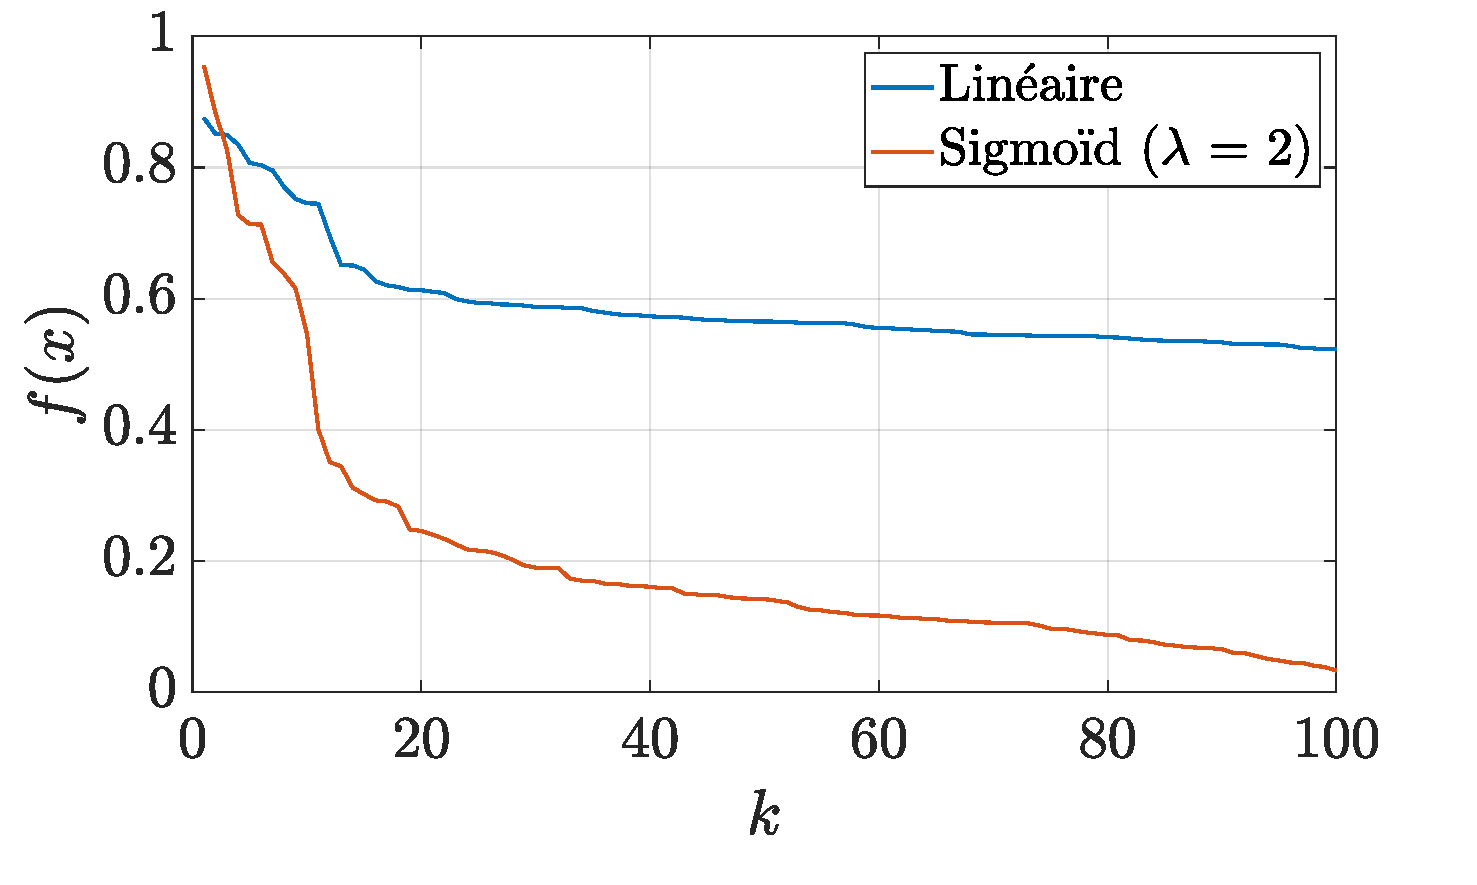
\includegraphics[width=0.7\linewidth]{./figures/NMF/lin_sig.pdf}
    \caption{Similarité cosinus pour une représentation linéaire et sigmoïdienne.}
    \label{fig:resume_simil}
\end{figure}

Le dictionnaire \textit{trafic}, $\mathbf{W}_{trafic}$, est ensuite défini en pondérant chaque base de $\mathbf{W'}$ par $\alpha$, un vecteur de pondération tel que : 

\begin{equation}
\mathbf{w}_{trafic} = \alpha_k \mathbf{w'}_k
\end{equation}

avec $\mathbf{\alpha}_{1 \times K} = \left[\alpha_1, \alpha_2 \dots \alpha_K \right]$ où $\alpha_k \in \left[0,1 \right]$. $\alpha_k$ est défini en fonction de la similarité entre $\mathbf{w_0}$ et $\mathbf{w'}$ à l'aide d'une méthode de seuillage. 2 méthodes sont envisagées : 

\begin{itemize}
\item le seuillage dur (\textit{hard thresholding}) \cite{donoho1994threshold} qui consiste à ne considérer que les éléments de $\mathbf{W'}$ dont la distance/similarité est supérieure à une valeur seuil $t$. 

\begin{subequations}\label{eq:seullageDur_def}
\begin{numcases}{\alpha_k =}
	0 & si \quad $f_{LIN/SIG}(k) \leq t_h$,  \\
	1 & si \quad $f_{LIN/SIG}(k) > t_h$, 
\end{numcases}
\end{subequations}

\item le seuillage \textit{firm} \cite{fornasier2008iterative} qui consiste à pondérer les éléments situé entre deux seuils $t_{f,1}$ et $t_{f,2}$ avec $t_{f,1} < t_{f,2}$ en les normalisant entre 1 et 0 : 


\begin{subequations}\label{eq:seuillageFirm_def}
\begin{numcases}{\alpha_k =}
    0, & \text{si}  $f_{LIN/SIG}(k) \leq t_{f,1}$, \\
    \mathcal{N}(f_{LIN/SIG}(k)), & \text{si}  $t_{f,1} < f_{LIN/SIG}(k) \leq t_{f,2}$,\\
    x, & \text{si}  $f_{LIN/SIG}(k) > t_{f,2}$.
\end{numcases}
\end{subequations}

\end{itemize}

\begin{figure}
\centering
	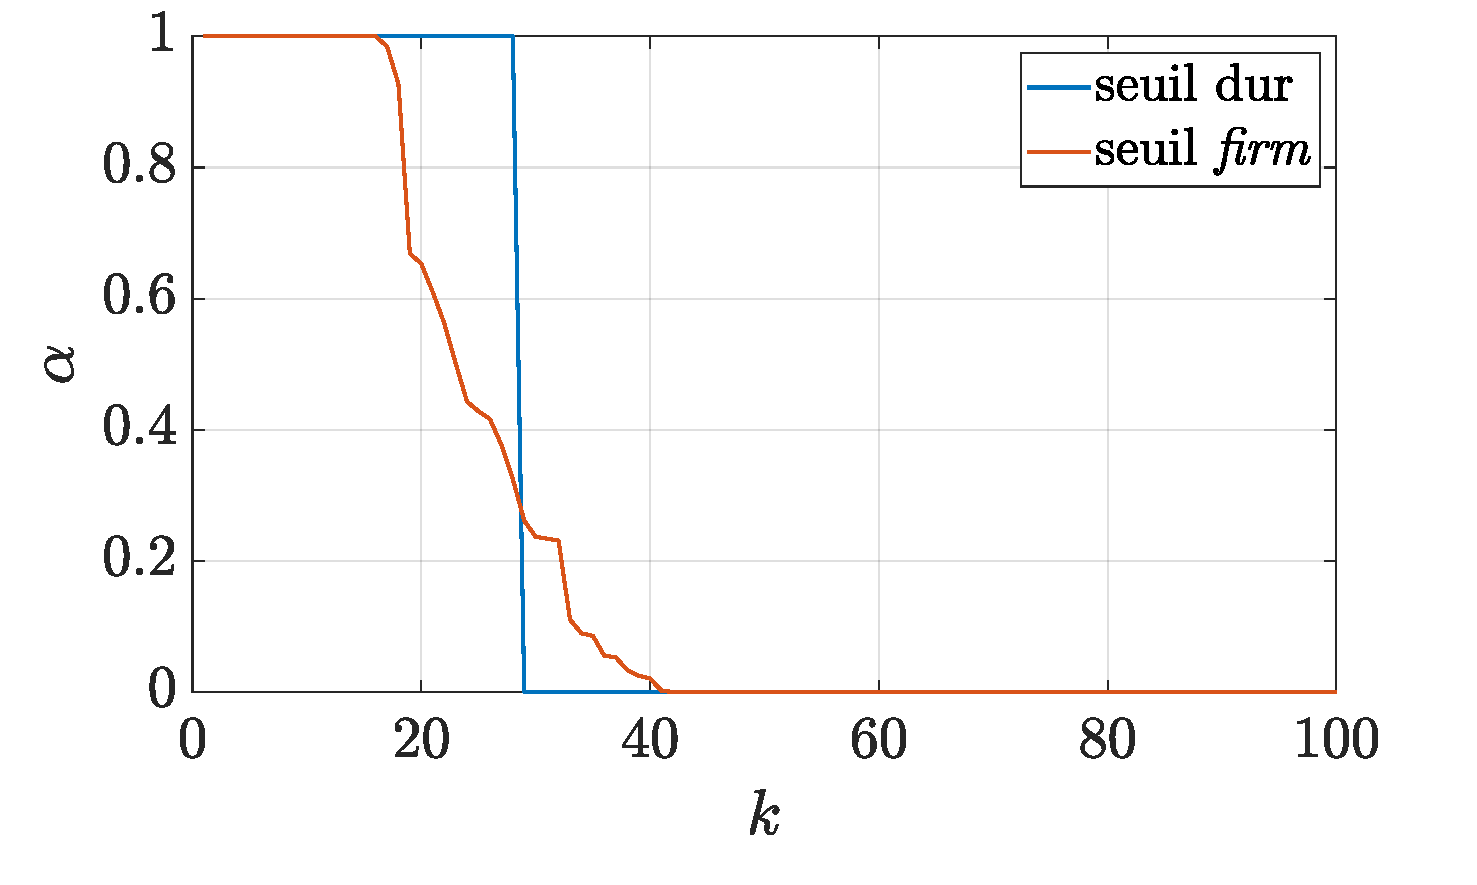
\includegraphics[width=.7\textwidth]{./figures/NMF/seuillage.pdf}
  \caption{Pondération $\alpha$ appliquée à $\mathbf{W'}$ composé de 100 bases avec pour seuil $t = 0,2$ (seuillage dur) et $t_{f,1} = 0,3$ et $t_{f,2} = 0,15$ (pour le seuillage \textit{firm})}
  \label{fig:seuillage}
\end{figure}

On résume les différentes étapes de cette étape au travers de l'algorithme

\begin{algorithm}
\caption{NMF initialisée seuillée}
\begin{algorithmic} 
\STATE Initialisation de $\mathbf{W_0}$
\FOR{i = 1 : nombre itération} 
	\STATE mise à jours de $\mathbf{W_0}$
	\STATE mise à jours de $\mathbf{H}$
\ENDFOR
\STATE Calcul de la similarité cosinus $D_{\theta}(\mathbf{W_0} \Vert \mathbf{W})$
\IF{représentation sigmoïde}
	\STATE $D_{\theta}(\mathbf{W_0} \Vert \mathbf{W}) = \sfrac{1}{\left(1+\exp({-\lambda D_{\theta}(\mathbf{W_0} \Vert \mathbf{W'})}\right)}$
\ENDIF

\IF{seuillage \textit{dur}} 
	\STATE $\alpha$ définit selon Eq. \ref{eq:seullageDur_def}
\ELSIF{seuillage \textit{firm}} 
	\STATE $\alpha$ définit selon Eq. \ref{eq:seuillageFirm_def}
\ENDIF
\STATE $\mathbf{W}_{trafic} = \alpha \mathbf{W'}$
\end{algorithmic}
\end{algorithm}


\section{NMF avec contraintes}\label{part:NMF_contrainte}
Si la NMF supervisée et semi-supervisée en elles seules offrent des résultats intéressants, de nombreux travaux se sont intéressés à contraindre l'allure du dictionnaire ou des activateurs suivant les connaissances\textit{a priori} de ces éléments. Ces contraintes sont alors pris en compte dans la fonction coût \ref{eq:costFunctionMM} par l'ajout d'un second terme pondéré $C(\mathbf{W},\mathbf{H})$, 
\begin{equation}
\underset{\textbf{W},\textbf{H}}{\text{min}}~D\left(\textbf{V} \vert\vert \textbf{WH}\right) + \alpha C(\mathbf{W},\mathbf{H}).
\end{equation}

Cette pénalité augmente alors la fonction coût si l'allure de $\mathbf{W}$ ou $\mathbf{H}$ n'est pas celle souhaitée. Le terme de pondération $\alpha$ permet alors de varier le poids de la contrainte : plus ce terme est grand et plus l'influence de la contrainte sera prépondérante. Plusieurs type de pénalités sont revues et serviront dans la suite de l'étude. 

\subsection{Contrainte de parcimonie}
Une des premières contraintes employées est celle de la parcimonie \cite{hoyer_non-negative_2004} \cite{le2015sparse} : c'est-à-dire l'utilisation d'un nombre réduit d'éléments du dictionnaire à chaque instant $t$. Cette contrainte renforce la représentation par partie de la NMF en pénalisant les termes qui serait non nul. Elle trouve notamment son intérêt dans le cas d'une représentation \textit{sur-complète} du dictionnaire, c'est à dire $K > \max(F,N)$ où l'ajout de contrainte parcimonieuse permet de réduire la complexité du problème. 

Dans un premier temps, Hoyer \cite{hoyer_non-negative_2004} propose une contrainte telle que 

\begin{equation}
C(h_k) = \frac{\sqrt{N}-\left( \sum_{n=1}^N \vert h_{kn} \vert \/ \sqrt{\sum_{n = 1}^N h_{kn}^2} \right)}{\sqrt{N}-1}
\end{equation}

qui équivaut au rapport de la norme $\ell_1$ et $\ell_2$ normalisée de $h_{kn}$. Ce rapport est ensuite défini tel que $C(h_k) = C_h$, une valeur constante définie qui fixe la quantité de parcimonie souhaitée dans $\mathbf{H}$. Un algorithme de gradient de descente permet ensuite , sous cette contrainte de résoudre l'équation \ref{eq:D(V-WH)}. Virtanen \cite{virtanen_monaural_2007} propose l'ajout d'une contrainte telle que $C_{sp}(\mathbf{h})$ est le plus souvent considéré comme la norme $\ell_1$ des éléments de $\mathbf{H}$,

\begin{equation}
C_{sp}(\mathbf{h}) = \sum_k h_{kn}
\end{equation}

La prise en compte de cette pénalisation  peut facilement être prise en compte dans les algorithmes de majorisation-minimisation : 

\begin{equation}\label{eq:derivé-fonc-auxiliaireSparse}
\nabla_{h_k} G(\mathbf{h}\vert \mathbf{\tilde{h}}) = \sum_f w_{fk}\left[\breve{d}'\left(v_f\vert \tilde{v_f}\frac{h_k}{\tilde{h}_k}\right) + \textit{\textroundcap{d}}'(v_f\vert \tilde{v_f})\right]+\lambda.
\end{equation}

L'algorithme de mise à jours de $\mathbf{H}$ devient alors 

\begin{subequations}
\begin{numcases}{h_k^{(i+1)} =}
    h_k^{(i)}\left(\frac{\sum_f w_{fk} v_f \tilde{v}_f^{(\beta-2)}}{\sum_f w_{fk} \tilde{v_f}^{(\beta-1)}+\lambda}\right)^{\gamma(\beta)}, & $\beta < 2$\label{eq:h_sparsity}\\
    h_k^{(i)}\left(\frac{\sum_f w_{fk} v_f \tilde{v}_f^{(\beta-2)}-\lambda}{\sum_f w_{fk} \tilde{v_f}^{(\beta-1)}}\right)^{\gamma(\beta)}, & $\beta \geq 2$.\label{eq:h_sparsity_2}
\end{numcases}
\end{subequations}

Dans le cas où $\beta \geq 2$, la contrainte apparait au numérateur et est soustractive. Ce comportement peut être problématique dans le cadre de la non-négativité suivant la value de $\alpha_{sp}$ \cite{fevotte_algorithms_2011}.

\subsection{Contraintes temporelles : \textit{smooth} NMF}

La mise à jour des activateurs temporelles dans la NMF supervisée et non-supervisée se fait trame par trame sans prendre en compte la corrélation qu'il puisse y avoir entre la trame $n$ et les trames précédentes. Néanmoins, la plupart des sons réels ont une évolution temporelle lente. Prendre en compte les trames temporelles précédentes permettrait que la forme des activateurs soient plus réalistes et proposerait un outil plus robuste dans la reconstruction du signal. Cette outil trouve son intéret dans la musique (\cite{virtanen_sound_2003}, \cite{fevotte_majorization-minimization_2011}) où les instruments (à l'exception des instruments percussifs) peuvent jouer des notes s'étalant sur plusieurs centaines de milli-secondes. Mais c'est aussi le cas au sein d'environnements sonores urbains où les sons (notamment le trafic routier) ont des variations lentes, de plusieurs secondes. Contraindre l'allure des activateurs à des formes lentes est donc sensé et pourrait s'assurer d'obtenir des formes d'activations plus réalistes. L'une des approches les plus citées est celle de Virtanen \cite{virtanen_monaural_2007} qui fut ensuite généralisé sous forme d'algorithme générique dans \cite{fevotte2017single}.  L'ajout de la contrainte se traduit par une modification de la fonction cout (équation \ref{eq:D(V-WH)}) : 

\begin{equation}\label{eq:CostSmoothEssid}
\underset{\mathbf{W}, \mathbf{H} > 0}{\text{min}}~ C(\mathbf{W},\mathbf{H}) = D(\mathbf{V}\vert\vert \mathbf{WH}) + C_t(\mathbf{H})
\end{equation}

avec $C_t(\mathbf{H})$, la contrainte temporelle
 
\begin{equation}
C_t(\mathbf{H}) = \sum_{n=1}^K \alpha_k\sum_{n=2}^N \left(h_{kn} - h_{k(n-1)})\right)^2
\end{equation}

où $\alpha_k$ est la pondération de la contrainte. Celle-ci peut être variable suivant $k$ ou bien constante sur tout les éléments ($\alpha_k = \alpha$). Par l'ajout de cette contrainte, les fortes variations d'un vecteur d'activation entre l'indice $n$ et $n-1$ sont donc pénalisante à travers l'utilisation de l'opérateur \textit{carré}. La mise à jours de $\mathbf{H}$, afin de minimiser la fonction cout, va alors privilégié les variations plus lentes pour réduire le poids de la contrainte $C_t$. L'algorithme de mise à jour devient :

\begin{equation}
\textbf{H}^{(i+1)} \leftarrow \textbf{H}^{(i)} \otimes\left(\frac{\textbf{W}^T \left[\left(\textbf{WH}^{(i)} \right)^{(\beta-2)} \otimes \textbf{V} \right] + 2 A \otimes \left(\overrightarrow{\mathbf{H}}^{(i)} + \overleftarrow{\mathbf{H}}^{(i)} \right)}{\textbf{W}^T \left[\textbf{WH}^{(i)} \right]^{(\beta-1)} + 2 A \otimes \left(\mathbf{H}^{(i)} + \overleftrightarrow{\mathbf{H}}^{(i)} \right)}\right)^{\gamma(\beta)}\label{eq:HupdateSmooth}
\end{equation}

avec 

\begin{subequations}
\begin{align}
    A &= 
\begin{bmatrix} 
\alpha_1 &  \cdots & \alpha_1  \\ 
\alpha_2 & \dots & \alpha_2  \\ 
\vdots & \ddots &  \vdots \\
\alpha_K & \cdots & \alpha_K
\end{bmatrix}, \label{eq:subeq1}\\
    \overrightarrow{\mathbf{H}} &= 
\begin{bmatrix}
0 & h_{1,1} & h_{1,2} & \cdots & h_{1,N-1}\\
0 & h_{2,1} & h_{2,2} & \cdots & h_{2,N-1}\\
\vdots & \vdots & \vdots & \ddots & \vdots\\
0 & h_{K,1} & h_{K,2} & \cdots & h_{K,N-1}\\
\end{bmatrix}, \label{eq:subeq2}\\
    \overleftarrow{\mathbf{H}} &= 
\begin{bmatrix}
h_{1,2} & h_{1,3} & \cdots & h_{1,N} & 0\\
h_{2,2} & h_{2,3} & \cdots & h_{2,N} & 0\\
\vdots & \vdots & \ddots & \vdots & \vdots\\
h_{K,2} & h_{K,3} & \cdots & h_{K,N} & 0\\
\end{bmatrix}, \label{eq:subeq3}\\
    \overleftrightarrow{\mathbf{H}} &= 
\begin{bmatrix}
0 & h_{1,2} & \cdots & h_{1,N-1} & 0\\
0 & h_{2,2} & \cdots & h_{2,N-1} & 0\\
\vdots & \vdots & ddots & \vdots & \vdots\\
0 & h_{K,2} & \cdots & h_{K,N-1} & 0\\
\end{bmatrix}. \label{eq:subeq5}
\end{align}
\end{subequations}

$A$ résume les valeurs des contraintes selon $k$, $\overrightarrow{\mathbf{H}}$, les valeurs de $\mathbf{H}$ à l'instant $n-1$, $\overleftarrow{\mathbf{H}}$, les valeurs de $\mathbf{H}$ à l'instant $n+1$ et enfin $\overleftrightarrow{\mathbf{H}}$, les valeurs de $\mathbf{H}$ sur l'intervalle $\left[2~N-1 \right]$. L'impact du coefficient de pondération $\alpha$ sur les activations de $\mathbf{H}$ est représenté en Figure \ref{fig:smoothnessExample}. Plus cette pondération est forte plus l'allure des activateurs est \textit{smooth} .

\begin{figure}[hbtp]
\centering
	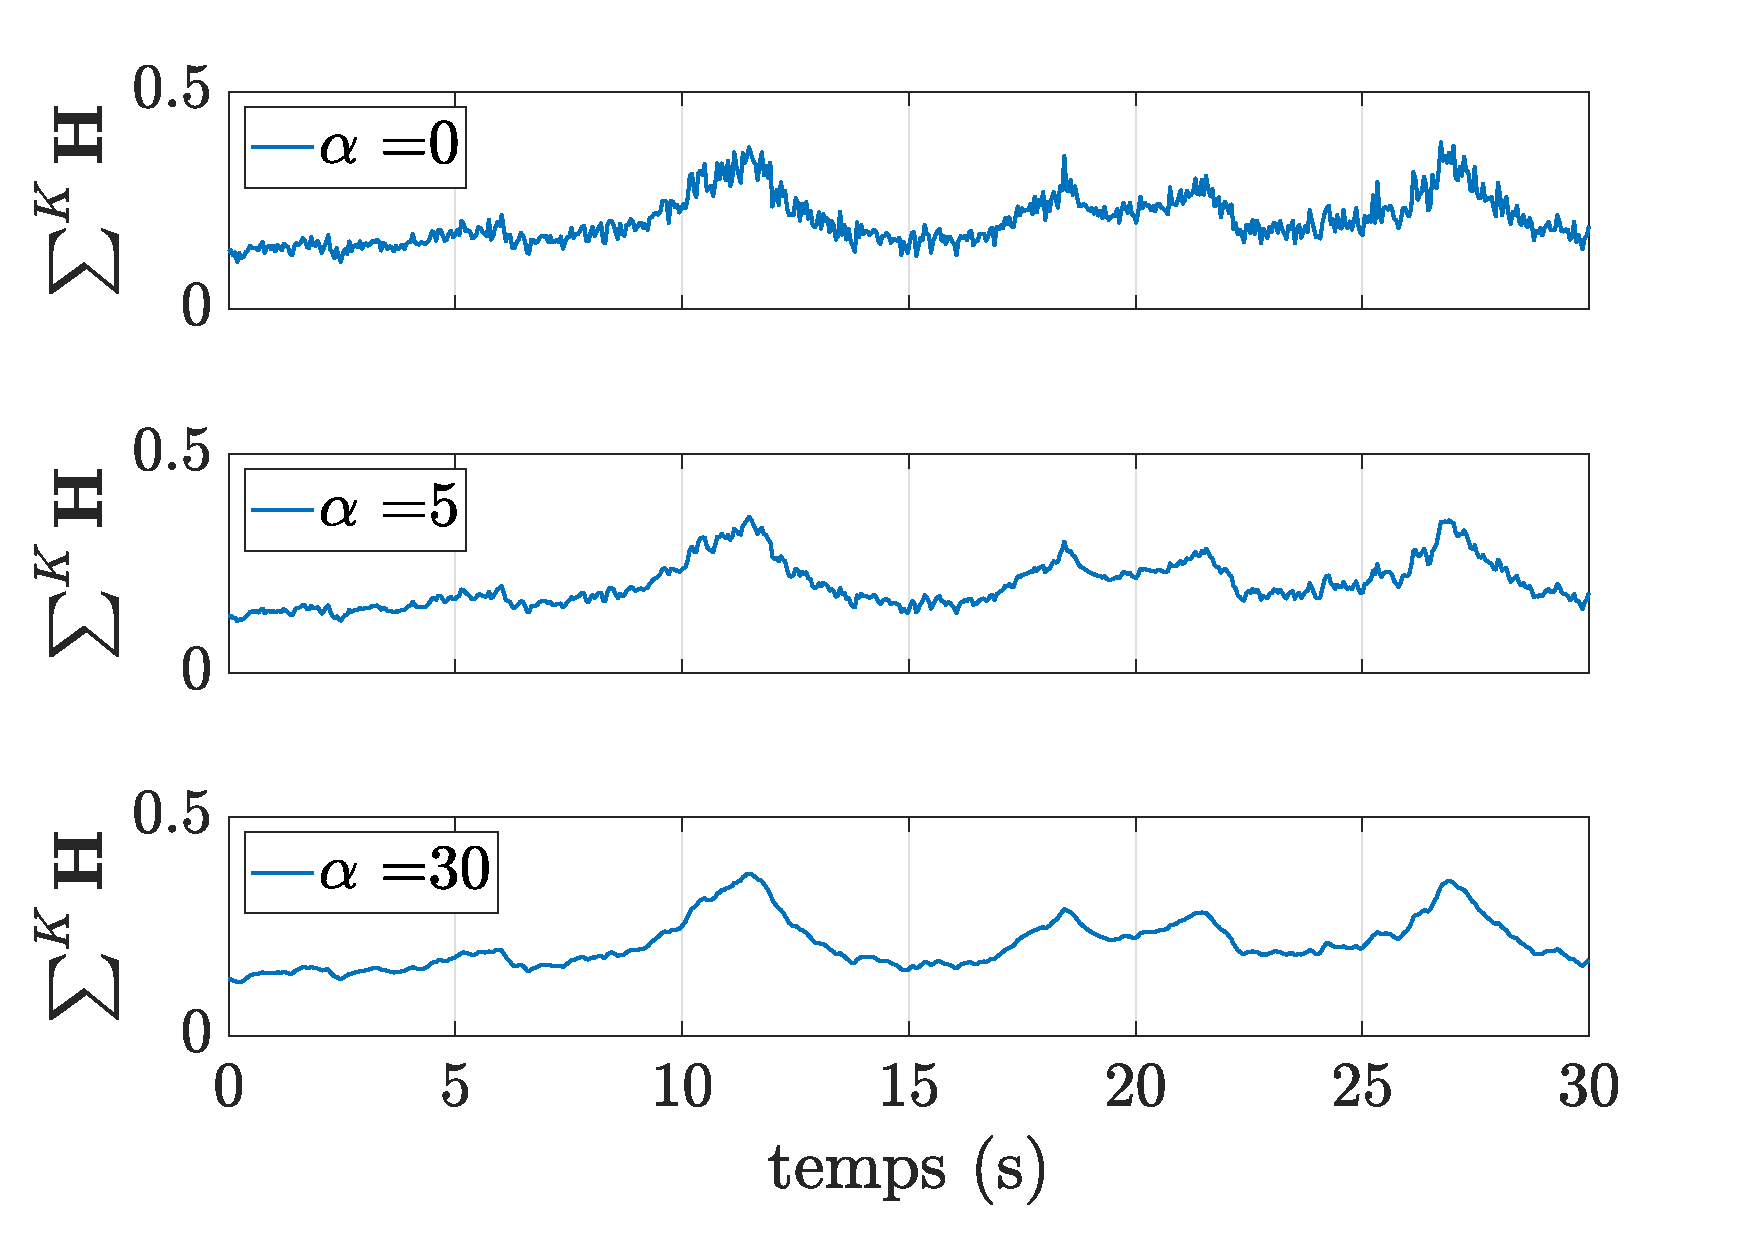
\includegraphics[width=0.7\linewidth]{./figures/NMF/smoothness_02.pdf}
\caption{Influence de la pondération sur la forme des activateurs sommés selon $K$ sur une scène de 30 secondes.}
\label{fig:smoothnessExample}
\end{figure}

\subsection{Autres contraintes}

D'autre contraintes existent et ne seront pas investigué tels que l'harmonicité du dictionnaire


\subsection{Contrainte sur le dictionnaire}

Dans le cas de la NMF semi-supervisée, les éléments libres de $\mathbf{W_r}$ ne sont soumis à aucune contrainte et peuvent donc y inclure des éléments qu'on ne souhaite pas trouver et \textit{in fine} dégrader la séparation de source. Dans notre cas, la reconstruction du signal \textit{trafic} ne faisant qu'avec $\mathbf{W_s}$, il faut s'assurer que les spectres de $\mathbf{W_r}$ ne contiennent pas d'informations de cette classe de son. En conséquence, comme les spectres \textit{trafic} sont surtout compris dans les basses fréquences ($\left[0-2000 \right]$ Hz), on choisit  de contraindre $\mathbf{W_r}$ afin que l'allure des spectres ne soit pas similaire à ceux de $\mathbf{W_s}$. Les travaux de Kitamura $\&$ al. \cite{kitamura} permettent d'inclure une contrainte qui permet d'inlcure la maximisation de la distance entre $\mathbf{W_s}$ et $\mathbf{W_r}$ à la fonction coût \ref{eq:D(V-WH)} : 

\begin{equation}
\underset{\mathbf{W}, \mathbf{H} > 0}{\text{min}}~ C(\mathbf{W},\mathbf{H}) = D(\mathbf{V}\vert\vert \mathbf{WH}) + \alpha_{ss} C_{ss}(\mathbf{W_s},\mathbf{W_r}).
\end{equation}

Le calcul de fonction coût pénalisée, $C_{ss}$ équivalent à  

\begin{align}
C_{ss}(\mathbf{W_s},\mathbf{W_r}) = \exp\left(-\frac{1}{\lambda_{ss}}\sum_{f,m,j}d_{\beta_{ss}}(w_{s_{fk}} \mid w_{r_{fj}})\right)
\end{align}

où $\alpha_{ss}$ est la pondération de la contrainte, $\lambda_{ss}$, un terme de sensitivité. $D_{\beta_{ss}}(x \mid y)$ est un calcul de divergence définit selon \ref{eq:divBetaGenerale} et qui dépend d'une valeur $\beta_{ss}$ qui n'a pas a être nécessairement égal au choix de $\beta$. Avec cette contrainte, plus $\mathbf{W_r}$ est différent de $\mathbf{W_s}$, plus la distance augmente et et plus $C_{ss}$ diminue.  L'expression de la matrice $\mathbf{W_r}$ est ensuite déterminée par la même approche que celle employée dans la partie \ref{part:sub_fonction_aux} : 

\begin{equation}
\mathbf{W_r}^{(i+1)} \leftarrow \mathbf{W_r}^{(i)}.\left(\frac{\lambda_{ss}\left[\left(\mathbf{\tilde{V}}^{(i)} \right)^{(\beta-2)}.\mathbf{V} \right]\mathbf{H_r}^T+\alpha_{ss}\left(\mathbf{W_r}^{(i)}\right)^{(\beta_m-1)}C_{ss}}{\lambda_{ss}\left(\mathbf{\tilde{V}}^{(i)} \right)^{(\beta-1)}\mathbf{H_r}^T+\alpha_{ss}\left(\mathbf{W_r}^{(i)}\right)^{(\beta_m-2)}C_{ss}\sum_k \mathbf{W_s}} \right)^{\gamma(\beta)}
\end{equation}

Les expressions des matrices $\mathbf{H_r}$ et $\mathbf{H_s}$ restent, quant à elles, inchangées (\ref{eq:H_r_SS}, \ref{eq:H_s_SS}). On illustre l'avantage de cette méthode par un cas simple où $\mathbf{W_s}$ n'est constitué que de spectres \textit{trafic} et une scène $\mathbf{V}$ comprend des éléments \textit{trafic} et \textit{oiseaux}. La figure où l'allure de $\mathbf{W_r}$ est comparé suivant que la contrainte soit présente ou non. La présence de la contrainte permet de s'assurer que $\mathbf{W_r}$ n'inclus que les éléments qui ne sont pas $\mathbf{W_s}$.\\

Cette contrainte n'est toutefois pas la seul qui existe, Duan $\&$ al. \cite{duan_online_2012}, via l'approche de la PLCA, décide dans un premier temps de détecter les évènements qui ne peuvent être reconnu par $\mathbf{W_s}$ pour ensuite apprendre $\mathbf{W_r}$ dessus. \cite{} dans le cas de la séparation entre une signal de parole et musical, ajoute une contrainte de parcimonie sur les éléments mobiles en vue d'y inclure des spectres harmoniques et donc ainsi les signaux musicaux.
 




%\appendix
%\chapter{Démonstration de la relation entre la distribution de Tweedie et les $\beta$-divergences}\label{annexe:tweedie}
%
%Pour déterminer la similarité de deux probabilités de distributions $x$ et $y$, l'approche statistique est considérée et notamment celle basée sur les modèles de dispersion exponenentielle définit par Jorgensen \cite{jorgensen_exponential_1987},  
%
%\begin{equation} \label{eq:Annexe_modele_disp_exp}
%p\left(x\vert \theta,\varphi\right) = h(x,\theta) \exp\left[\lambda^{-1}\left(\theta x-\psi(\theta) \right)\right], 
%\end{equation}
%
%avec $h(x,\theta) $, la mesure de base, $\theta$, le paramètre normal (ou canonique), $\lambda$, celui de la dispersion et $\psi$ celui de la normalisation. .  
%La moyenne (ou espérance) est dénommée $\mu$ et est liée à $\theta$ par les relations~\ref{eq:mu1} et \ref{eq:mu2}.
%
%\begin{equation}\label{eq:eq:Annexe_mu1}
%\mu(\theta) = \frac{d\varphi(\theta)}{d\theta}
%\end{equation}
%\begin{equation}\label{eq:eq:Annexe_mu2}
%\theta(\mu) = \frac{d\phi(\mu)}{d\mu}
%\end{equation}
%
%On observe que $\phi(\mu)$ est le conjugué dual de $\varphi(\theta)$ tout comme $\theta$ et $\mu$. \cite{Jorgensen} donne une relation directe liant ces deux dernières grandeurs,  
%
%\begin{equation}\label{eq:eq:Annexe_theta}
%\frac{d\theta}{d\mu} = \upsilon(\mu)^{-1}, 
%\end{equation}
%
%avec $\upsilon$ la fonction variance, elle même lié à la variance de la distribution par le paramètre de dispersion : 
%
%\begin{equation}
%Var(x) = \lambda \upsilon(\mu).
%\end{equation}
%
%La distribution de Tweedie est alors définit comme un cas particulier des Modèles de Dispersion Exponentielles lorsque la variance est liée à la moyenne par la puissance $n$ (\ref{eq:Tweedie})
%\begin{equation}\label{eq:eq:Annexe_Tweedie}
%\upsilon(\mu) = \mu^n \quad \text{avec $n \in \mathbb{N}$.}
%\end{equation}
%
%Le choix de la puissance $n$ influe sur celui de la distribution des données (voir Tableau~\ref{tab:puissance_p} pour les distributions les plus couramment utilisées). Par exemple, dans le cas d'une loi normale ($n = 0$), l'expression de la distribution de probabilité \ref{eq:modele_disp_exp} s'exprime par
%
%\begin{equation}\label{eq:eq:Annexe_distributionProbabilité}
%p(x;\mu,\sigma^2) = \frac{1}{\sigma\sqrt{2\pi}}\exp\left(\sfrac{\left(x-\mu \right)^2}{2\sigma^2} \right)
%\end{equation}
%
%qui s'exprime sous la forme d'une distribution de Tweedie
%
%\begin{equation}
%p(x;\mu,\sigma^2) = \frac{1}{\sigma\sqrt{2\pi}}\exp\left(\frac{-x^2}{2\sigma^2} \right)
%\exp\left(\frac{\left(x\mu-\sfrac{\mu^2}{2} \right)}{\sigma^2}\right)
%\end{equation}
%
%avec $\mu = \theta$, $\psi(\theta) = \dfrac{\mu^2}{2}$, $\lambda = \sigma^2$ où $\sigma$ est l'écart-type et $h(x,\lambda) = \sqrt{\dfrac{1}{\lambda 2\pi}}e^{\sfrac{-x^2}{2}}$.\\
%
%\begin{table}[H] 
%\centering
%	\begin{tabular}{cccc}
% 		\hline			
%   		$n$ & 0 & 1 & 2 \\
%   		\hline
%   		distribution & Gaussienne & Poisson & Gamma\\
%   		\hline
% 	\end{tabular}
%\caption{relation entre plusieurs valeurs de la puissance $p$ et la distribution de données}
%\label{tab:eq:Annexe_puissance_p}
%\end{table}
%
%Des relations \ref{eq:mu2}, \ref{eq:theta},  \ref{eq:Tweedie} et d'un changement de variable, $\beta = 2-p$, l'expression de la fonction cumulante dual $\phi_{\beta}(\mu)$ est déterminée : 
%
%\begin{subequations}\label{eq:eq:Annexe_gamma_beta}
%\begin{numcases}{\phi_{\beta}(\mu)=}
%    \frac{\mu^{\beta}}{\beta(\beta-1)}-\frac{\mu}{\beta-1}+\frac{1}{\beta}, & $\beta \in \mathbb{R} \backslash \lbrace 0,1\rbrace$,\label{eq:eq:Annexe_phi}\\
%    -\log \mu + \mu - 1, & $\beta = 0$,\label{eq:eq:Annexe_phiIs}\\
%    \mu\log \mu - \mu + 1, & $\beta = 1$.\label{eq:eq:Annexe_phiKL}
%\end{numcases}
%\end{subequations}
%Les cas \ref{eq:phiIs} et \ref{eq:phiKL} correspondent au cas limite de \ref{eq:phi}. Ces fonctions sont continues pour $\mu \in \left[0 +\infty \right[$, deux fois dérivables au voisinage de $\mu = 1$ ($\phi(1) = \phi'(1) = 0$ et $\phi''(1) = 1$) définissant un ensemble de fonctions convexes satisfaisant les conditions pour être utilisables au sein des divergences de Bregman.\\
%
%\chapter{Smooth NMF based on \cite{essid_smooth_2013} for $\beta = 2$}
%
%mais c'est l'approche proposée par Essid et Févotte \cite{essid_smooth_2013} qui est retenu ici.\\
%
%Leur méthode, proposée dans le cadre de la structuration automatique de documents audiovisuels, a pour forme

%%%%%%%%%%%%%%%%%%%%%%%%%%%%%%%%%%%%%%%%%%%%%%%%%%%
%\bibliographystyle{unsrt}
%\bibliography{../bibliographie}
%
%\end{document}